\documentclass[a4paper, 10pt, twoside]{article}

\usepackage[top=1in, bottom=1in, left=1in, right=1in]{geometry}
\usepackage[utf8]{inputenc}
\usepackage[spanish, es-ucroman, es-noquoting, activeacute]{babel}
\usepackage{setspace}
\usepackage{fancyhdr}

\usepackage{lastpage}
\usepackage{amsmath}
\usepackage{amsfonts}
\usepackage{amsthm}
\usepackage{verbatim}
\usepackage{fancyvrb}
\usepackage{graphicx}
\usepackage{float}
\usepackage{enumitem} % Provee macro \setlist
\usepackage{tabularx}
\usepackage{multirow}
\usepackage{hyperref}
\usepackage{xspace}
\usepackage{qtree}
\usepackage[toc, page]{appendix}
\usepackage{enumitem}
\usepackage{userStories}


%%%%%%%%%% Constantes - Inicio %%%%%%%%%%
\newcommand{\titulo}{Trabajo Práctico 1}
\newcommand{\materia}{Ingeniería de Software II}
\newcommand{\integrantes}{Almansi, Gasperi Jabalera, Russo, Tagliavini}
\newcommand{\cuatrimestre}{Primer Cuatrimestre de 2016}
%%%%%%%%%% Constantes - Fin %%%%%%%%%%


%%%%%%%%%% Configuración de Fancyhdr - Inicio %%%%%%%%%%
\pagestyle{fancy}
\thispagestyle{fancy}
\lhead{\titulo\ · \materia}
\rhead{\integrantes}
\renewcommand{\footrulewidth}{0.4pt}
\cfoot{\thepage /\pageref{LastPage}}

\fancypagestyle{caratula} {
   \fancyhf{}
   \cfoot{\thepage /\pageref{LastPage}}
   \renewcommand{\headrulewidth}{0pt}
   \renewcommand{\footrulewidth}{0pt}
}
%%%%%%%%%% Configuración de Fancyhdr - Fin %%%%%%%%%%


%%%%%%%%%% Miscelánea - Inicio %%%%%%%%%%
% Evita que el documento se estire verticalmente para ocupar el espacio vacío
% en cada página.
\raggedbottom

% Separación entre párrafos.
\setlength{\parskip}{0.5em}

% Separación entre elementos de listas.
\setlist{itemsep=0.5em}

% Asigna la traducción de la palabra 'Appendices'.
\renewcommand{\appendixtocname}{Apéndices}
\renewcommand{\appendixpagename}{Apéndices}

\newcommand{\grafico}[1]{
  \begin{center}
    \includegraphics[width=15cm]{#1}
  \end{center}
}


%%%%%%%%%% Miscelánea - Fin %%%%%%%%%%


%%%%%%%%%% User stories y tareas - Inicio %%%%%%%%%%
% Entorno dentro del cual se declaran las stories del product backlog con el
% macro \story.
\newenvironment{stories}{
  \begin{itemize}
}{
  \end{itemize}
}

% Uso: \story{id}{rol}{historia}{criterio de aceptación}.
\newcommand{\story}[4]{
  \item
  \textbf{ID #1:} Como \emph{#2} quiero \emph{#3} para \emph{#4}.
}

% Uso: \sprintstory{id}{rol}{historia}{criterio de aceptación}.
\newcommand{\sprintstory}[4]{
  \noindent
  \textbf{ID #1:} Como \emph{#2} quiero \emph{#3} para \emph{#4}.
}

% Entorno dentro del cual se declaran los detalles de un story con el macro
% \detalle.
\newenvironment{detalles}{
  \textbf{Detalles:}
  \begin{itemize}
}{
  \end{itemize}
}

% Uso: \detalle{un detalle de la story}
\newcommand{\detalle}[1] {
  \item #1.
}

% Entorno dentro del cual se declaran los criterios de aceptación de un story
% con el macro \criterio.
\newenvironment{criterios}{
  \textbf{Criterio de aceptación:}
  \begin{itemize}
}{
  \end{itemize}
}

% Uso: \criterio{criterio de aceptación}
\newcommand{\criterio}[1] {
  \item #1
}

% Entorno dentro del cual se declaran las tareas de un story con el macro \task.
\newenvironment{tasks}{
  \textbf{Tareas:}
  \begin{enumerate}
}{
  \end{enumerate}
}



\begin{document}


%%%%%%%%%%%%%%%%%%%%%%%%%%%%%%%%%%%%%%%%%%%%%%%%%%%%%%%%%%%%%%%%%%%%%%%%%%%%%%%
%% Carátula                                                                  %%
%%%%%%%%%%%%%%%%%%%%%%%%%%%%%%%%%%%%%%%%%%%%%%%%%%%%%%%%%%%%%%%%%%%%%%%%%%%%%%%


\thispagestyle{caratula}

\begin{center}


\includegraphics[height=2cm]{DC.png} 
\hfill

\includegraphics[height=2cm]{UBA.jpg} 

\vspace{2cm}

Departamento de Computación,\\
Facultad de Ciencias Exactas y Naturales,\\
Universidad de Buenos Aires

\vspace{4cm}

\begin{Huge}
\titulo
\end{Huge}

\vspace{0.5cm}

\begin{Large}
\materia
\end{Large}

\vspace{1cm}

\cuatrimestre

\vspace{4cm}

\begin{tabular}{|c|c|c|}
\hline
Apellido y Nombre & LU & E-mail\\
\hline
Almansi, Emilio Guido          & 674/12         & ealmansi@gmail.com\\
Gasperi Jabalera, Fernando     & 56/09            & fgasperijabalera@gmail.com\\
Christian ``El Capo del Sorting'' Russo               & 679/10         & christian.russo8@gmail.com\\
Tagliavini Ponce, Guido       & 783/11            & guido.tag@gmail.com\\
\hline
\end{tabular}

\end{center}

\newpage

\tableofcontents

\newpage


%%%%%%%%%%%%%%%%%%%%%%%%%%%%%%%%%%%%%%%%%%%%%%%%%%%%%%%%%%%%%%%%%%%%%%%%%%%%%%%
%% Introducción                                                              %%
%%%%%%%%%%%%%%%%%%%%%%%%%%%%%%%%%%%%%%%%%%%%%%%%%%%%%%%%%%%%%%%%%%%%%%%%%%%%%%%


\section{Introducción}

El actual informe presenta el an\'alisis y desarrollo inicial realizado para el producto \textbf{The Curry Game}. En el mismo se detallan el conjunto de user stories que abarcan el desarrollo completo de la aplicaci\'on, incluyendo tanto las definiciones actuales como los puntos de extensi\'on que se tendr\'an en cuenta. 
El objetivo de la aplicaci\'on es que los usuarios puedan armar sus equipos de basket, pudiendo participar de desaf\'ios entre los usuarios con el fin de ganar mas fichas que le permiten armar un mejor y m\'as robusto equipo. 
El sistema cuenta con una simulaci\'on del juego, que provee un log para poder ver c'omo se desarrolla el juego.


\subsection{Roles de usuario}

Por brevedad, se utilizan los siguientes roles en las User Stories a lo largo de este trabajo:

\begin{description}
  \item[Jugador:] cualquier usuario del sistema.

  \item[Participante:] un jugador que postula o acepta un desaf\'io.

  \item[Game designer:] el encargado de determinar los detalles de la simulaci\'on.


\end{description}

\subsection{Observaciones}
La herramienta de planificaci\'on \'agil elegida por el equipo es \textbf{TargetProcess}. Esta herramienta utiliza un sistema de ranking para el Business Value muy particular, que nosotros traducimos en valores entero del 1 al 4 del siguiente modo:
\begin{itemize}
    \item Must Have: 4
    \item Great: 3
    \item Average: 2
    \item Nice To Have: 1
\end{itemize} 

Utilizamos Spikes para mostrar las tareas preliminares. 
Por otro lado, luego de hacer un an\'alisis del sistema se decidi\'o que el lenguaje de programaci\'on que utilizaremos ser\'a Python, que es de f'acil utilizaci'on para programaci'on de prop'osito general (como programar el simulador en cuesti'on) y provee una sencilla API para realizar solicitudes HTTP.

%%%%%%%%%%%%%%%%%%%%%%%%%%%%%%%%%%%%%%%%%%%%%%%%%%%%%%%%%%%%%%%%%%%%%%%%%%%%%%%
%% Product backlog                                                           %%
%%%%%%%%%%%%%%%%%%%%%%%%%%%%%%%%%%%%%%%%%%%%%%%%%%%%%%%%%%%%%%%%%%%%%%%%%%%%%%%

\section{Product Backlog}
En esta secci\'on se listan todas las User Stories del Backlog de nuestro sistema.

\subsection{Spikes}

\begin{enumerate}
    \item Investigar sobre qu\'e lenguaje es el m\'as adecuado para implementar el sistema. \textbf{(Horas Hombres: 2)}
    \item Investigar la API de la NBA para evaluar la dificultad de implementar la lectura autom\'atica de datos de jugadores. \textbf{(Horas Hombres: 2)}
    \item Investigar la API de Twitter para evaluar la dificultad de implementar la medici\'on de popularidad de un jugador en Twitter. \textbf{(Horas Hombres: 1)}
    \item Instalar un entorno de desarrollo \textbf{(Horas Hombres: 2)}
    \item Instalar un entorno de testing  \textbf{(Horas Hombres: 3)}
\end{enumerate}


\subsection{Product backlog}
\subsubsection{Turnos}
\begin{enumerate}
    \item Como game designer quiero que el juego tenga 40 turnos.
    \\SP: 1, BV: 4
    \item Como game designer quiero que al empezar cada turno, un equipo comience atacando y el otro defendiendo.
    \\SP: 1, BV: 4
    \item Como game designer quiero que al empezar cada turno, el equipo que comienza atacando se vaya alternando entre ambos equipos.
    \\SP: 2, BV: 4
    \item Como game designer quiero que al empezar el primer turno, el equipo atacante sea elegido al azar.
    \\SP: 2, BV: 4
    \item Como game designer quiero que los turnos acaben si la pelota se va de la cancha o si se realiza un tiro exitoso al aro.
    \\SP: 3, BV: 4
    \item Como game designer quiero que, en caso de que se agoten los turnos y ambos equipos tengan el mismo puntaje, se jueguen 6 turnos extra de pr\'orroga.
	\\SP: 3, BV: 4
\subsubsection{Sobre un Jugador}
    \item Como game designer quiero que un jugador en ataque pueda lanzar la pelota al aro (por 2 o 3 puntos) o intentar un pase, y s\'olo eso.
    \\SP: 3, BV: 4
    \item Como game designer quiero que un jugador en defensa pueda intentar bloquear tiros al aro de otro jugador. 
     \\SP: 3, BV: 4
    \item Como game designer quiero que un jugador en defensa pueda interceptar pases.
    \\SP: 8, BV: 4
    \subsubsection{Puntos}
        \item Como game designer quiero que cuando un jugador realice un tiro al aro con \'exito, su equipo sume 2 o 3 puntos seg\'un corresponda.
    \\SP: 2, BV: 4
\subsubsection{Rebotes y pelotas divididas}
    \item Como game designer quiero que cuando cuando un tiro al aro resulte fallido o bloqueado, la pelota quede dividida y ambos equipos tengan la posibilidad de recuperarla.
    \\SP: 2, BV: 4
    \item Como game designer quiero que cuando una pelota quede dividida, la misma se dispute en forma intercalada entre los jugadores del equipo defensivo y del equipo ofensivo, en orden decreciente seg\'un n\'umero de posici\'on.
    \\SP: 5, BV: 4
    \item Como game designer quiero que cuando un jugador defensor gane una pelota dividida, se inviertan los roles de atacante y defensor entre ambos equipos.
    \\SP: 3, BV: 4
    \item Como game designer quiero que cuando un jugador atacante gane una pelota dividida, contin\'ue atacando su equipo.
    \\SP: 3, BV: 4
    \item Como game designer quiero que cuando ante una pelota dividida ninguno de los 10 jugadores gana el rebote, entonces la pelota salga de la cancha.
    \\SP: 3, BV: 4
    \subsubsection{Pases y robos de pelota}
    \item Como game designer quiero que cuando un jugador realice un pase de pelota exitoso y sin intercepci\'on, aumente en un peque\~no porcentaje la chance de \'exito de tiro al aro del jugador que realiza el tiro posteriormente en la jugada.
    \\SP: 1, BV: 4
    \item Como game designer quiero que cuando un jugador defensor tenga \'exito interceptando un pase, se cambien los roles de atacante y defensor entre los equipos y contin\'ue como atacante el equipo del defensor que rob\'o la pelota.
    \\SP: 3, BV: 4
    \item Como game designer quiero que cuando un pase sea fallido y adem\'as no sea interceptado por un defensor contrario, la pelota salga de la cancha.
    \\SP: 5, BV: 4
    \subsubsection{Sobre el equipo (DT y libro de jugadas)}
    \item  Como game designer quiero que el t\'ecnico tenga un libro de jugadas para jugar adecuadamente.
    \\SP: 3, BV: 4
    \item Como game designer quiero que el t\'ecnico tenga una frecuencia para cada jugada del libro para para poder ejecutarlas como si \'el lo hiciera.
    \\SP: 2, BV: 4
    \item  Como game designer quiero que al comenzar el ataque de un equipo (ya sea al iniciar un turno, recuperar una pelota dividida, o interceptar un pase), se elija una jugada ofensiva del libro de jugadas del director t\'ecnico del equipo atacante, teniendo en cuenta la frecuencia asignada a las mismas.
    \\SP: 2, BV: 4
    \item Como game designer quiero que cuando el equipo atacante elija una jugada ofensiva, el equipo defensor escoja una jugada defensiva de su libro de jugadas, teniendo en cuenta la frecuencia asignada a las mismas.
    \\SP: 2, BV: 4
    \subsubsection{Jugadas}
    \item Como game designer quiero que se pueda usar la jugada ofensiva colectiva externa. 
    \\SP: 3, BV: 4
    \item Como game designer quiero que se pueda usar la jugada ofensiva colectiva interna.
    \\SP: 3, BV: 4
    \item Como game designer quiero que se pueda usar la jugada ofensiva MVP.
    \\SP: 3, BV: 4
    \item Como game designer quiero que se pueda usar la jugada ofensiva Contra Ataque.
    \\SP: 3, BV: 4
    \item Como game designer quiero que se pueda usar la jugada defensiva Hombre a Hombre.
    \\SP: 3, BV: 4
    \item Como game designer quiero que se pueda usar la Dos Cada.
    \\SP: 5, BV: 4
    \item Como game designer quiero que se pueda usar la FiboJugada.
    \\SP: 5, BV: 4
    \subsubsection{F\'ormulas de resoluci\'on de acciones}
    \item Como game designer quiero que cada UE de una acci\'on X sea la probabilidad de \'exito al realizar la acci\'on X.
    \\SP: 3, BV: 4
    \item Como game designer quiero que el Umbral de Exito (UE) de tiro por 2 puntos sea FG para hacer el juego m\'as realista.
    \\SP: 2, BV: 4
    \item Como game designer quiero que el Umbral de Exito (UE) de tiro por 3 puntos sea 3P para hacer el juego m\'as realista.
    \\SP: 2, BV: 4
    \item Como game designer quiero que el Umbral de Exito (UE) de bloqueo sea  BPG * 0.2 para hacer el juego m\'as realista.
    \\SP: 2, BV: 4
    \item Como game designer quiero que el Umbral de Exito (UE) de pase de pelota sea 1 - TO * 0.1 para hacer el juego m\'as realista.
    \\SP: 2, BV: 4
    \item Como game designer quiero que el Umbral de Exito (UE) de robo de pelota sea SPG * 0.2 para hacer el juego m\'as realista.
    \\SP: 2, BV: 4
    \item Como game designer quiero que el Umbral de Exito (UE) de reboteo de pelota sea RPG * 0.05 para hacer el juego m\'as realista.
    \\SP: 2, BV: 4
    \item Como game designer quiero tener las estad\'isticas originales de los jugadores para que la simulaci\'on sea m\'as realista.
    \\SP: 13, BV: 4
    \item Como game designer quiero que la popularidad en Twitter de los jugadores para afecte mejorar su performance.
    \\SP: 13, BV: 4
    \subsubsection{Otras}
    \item Como jugador quiero armar un equipo para jugar en un desaf\'io.
    \\SP: 5, BV: 3
    \item Como jugador quiero aceptar un desaf\'io para ganar ranking, fichas y cap.
    \\SP: 8, BV: 3
    \item Como jugador quiero postular un desaf\'io para ganar ranking, fichas y cap.
    \\SP: 8, BV: 3
    \item Como participante de desaf\'io quiero en caso de ganar quiero que incremente mi n\'umero de fichas para tener m\'as fichas que otros jugadores y as\'i estar mejor posicionado en el ranking.
    \\SP: 1, BV: 3
    \item Como participante de desaf\'io quiero en caso de ganar quiero que incremente mi cap para poder formar mejores equipos.
    \\SP: 1, BV: 3
    \item Como participante de desaf\'io quiero apostar fichas.
    \\SP: 3, BV: 3
    \item Como participante de desaf\'io quiero que me resten las fichas que apost\'e.
    \\SP: 2, BV: 3
    \item Como participante de desaf\'io quiero elegir mi equipo para jugar con los jugadores que considere m\'as adecuados.
    \\SP: 5, BV: 3
    \item Como participante de desaf\'io quiero elegir mi DT para ejecutar las jugadas deseadas.
    \\SP: 3, BV: 3
    \item Como jugador quiero registrarme con mis datos para darme de alta en el sistema.
    \\SP: 8, BV: 3
    \item Como jugador quiero acceder a una tabla de rankings en base a cantidad de desaf\'ios ganados para informarme.
    \\SP: 8, BV: 2
    \item Como jugador quiero acceder a una tabla de rankings en base a cantidad de fichas total para informarme.
    \\SP: 8, BV: 2
    \item  Como jugador quiero poder guardar cada equipo que arme para usarlo luego en un desaf\'io.
    \\SP: 5, BV: 2
    \item Como jugador quiero autenticar mi email para activar mi cuenta.
    \\SP: 5, BV: 2
    \item Como jugador quiero loguearme con mi email (o username) para ingresar al sistema.
    \\SP: 8, BV: 2
    \item  Como jugador quiero obtener una cantidad inicial de fichas para apuestas para poder apostar.
    \\SP: 1, BV: 2
    \item Como jugador quiero obtener una cantidad de presupuesto (cap) inicial para poder armar mi equipo.
    \\SP: 1, BV: 2
    
\end{enumerate}
 
\section{Sprint backlog}
En esta secci\'on listamos un subconjunto de las User Stories del Backlog que decidimos meter dentro del Sprint teniendo en cuenta el Business Value. Para cada User Story detallamos descripci\'on, tareas, criterios de aceptaci\'on, etc.

% ********** US1 **************
\userStory	{US1} % ID en el Rally
	{Como game designer quiero que el juego tenga 40 turnos.} % titulo
	{Cada juego tendr\'a un total de 40 turnos.
  \\
  \\
\textbf{Criterios de aceptación:}\\
  \\
1. La cantidad de turnos que se muestran en el log es igual a 40.  \\
} % descripcion
	{} % criterios de aceptacion
	{1.0} % story points
	{Martin M} % story owner
	{Primera} % iteracion (Primera o ``no definida'')
	{Accepted} % estado (completada, bloqueada, etc.)

	\task	{Tarea1A} % ID en el Rally
		{Setear la cantidad inicial de iteraciones a 40.} % titulo
		{} % descripcion
		{0.25} % horas estimadas
		{} % story owner
		{} % horas faltantes
		{} % estado (completada, bloqueada, etc.)

	\task	{Tarea1B} % ID en el Rally
		{Testear que la cantidad de iteraciones este seteada en 40.} % titulo
		{} % descripcion
		{0.25} % horas estimadas
		{} % story owner
		{} % horas faltantes
		{} % estado (completada, bloqueada, etc.)
\vspace{20pt}


% ********** US2 **************
\userStory	{US2} % ID en el Rally
	{Como game designer quiero que al empezar cada turno, un equipo comience atacando y el otro defendiendo.} % titulo
	{En cada turno uno de los equipos comienza atacando y el otro defendiendo.
 \\
  \\
  \\
\textbf{Criterios de aceptación:}\\
  \\
1. En el log se notar\'a que al comienzo de un turno con dos equipos, uno de los equipos es atacante y el otro es defensor.  \\
} % descripcion
	{} % criterios de aceptacion
	{1.0} % story points
	{Martin M} % story owner
	{Primera} % iteracion (Primera o ``no definida'')
	{Accepted} % estado (completada, bloqueada, etc.)

	\task	{Tarea2A} % ID en el Rally
		{Diseñar un modelo donde se cuente con el equipo atacante y el equipo defensor} % titulo
		{} % descripcion
		{1.0} % horas estimadas
		{} % story owner
		{} % horas faltantes
		{} % estado (completada, bloqueada, etc.)

	\task	{Tarea2B} % ID en el Rally
		{Al comenzar un turno setear el equipo atacante y el defensor.} % titulo
		{} % descripcion
		{0.5} % horas estimadas
		{} % story owner
		{} % horas faltantes
		{} % estado (completada, bloqueada, etc.)

	\task	{Tarea2C} % ID en el Rally
		{Testear que en cada turno existe un equipo atacante y otro equipo defensor.} % titulo
		{} % descripcion
		{0.25} % horas estimadas
		{} % story owner
		{} % horas faltantes
		{} % estado (completada, bloqueada, etc.)
\vspace{20pt}


% ********** US3 **************
\userStory	{US3} % ID en el Rally
	{Como game designer quiero que al empezar cada turno, el equipo que comienza atacando se vaya alternando entre ambos equipos.} % titulo
	{Luego de cada turno el equipo que comenz\'o atacando en el turno anterior empezará defendiendo en el pr\'oximo.
\\
  \\
  \\
\textbf{Criterios de aceptación:}\\
  \\
1. En el log se notar\'a que en dos turnos consecutivos el equipo atacante no es el mismo. \\
2. En el log se notará que si en un turno un equipo atac\'o, en el pr\'oximo aparece defendiendo. \\
} % descripcion
	{} % criterios de aceptacion
	{2.0} % story points
	{Martin M} % story owner
	{Primera} % iteracion (Primera o ``no definida'')
	{Accepted} % estado (completada, bloqueada, etc.)

	\task	{Tarea3A} % ID en el Rally
		{Guardar el equipo que comienza atacando antes de comenzar un turno.} % titulo
		{} % descripcion
		{0.25} % horas estimadas
		{} % story owner
		{} % horas faltantes
		{} % estado (completada, bloqueada, etc.)

	\task	{Tarea3B} % ID en el Rally
		{Cuando termina un turno se setea al equipo que empezar\'a atacando en el pr\'oximo turno, como el equipo contrario al que empez\'o en el anterior.} % titulo
		{} % descripcion
		{0.5} % horas estimadas
		{} % story owner
		{} % horas faltantes
		{} % estado (completada, bloqueada, etc.)

	\task	{Tarea3C} % ID en el Rally
		{Diseñar un modelo en el cual el jugador atacante se valla alternando en cada turno.} % titulo
		{} % descripcion
		{0.5} % horas estimadas
		{} % story owner
		{} % horas faltantes
		{} % estado (completada, bloqueada, etc.)

	\task	{Tarea3D} % ID en el Rally
		{Testear que cuando pasa un turno el jugador atacante sea el otro equipo} % titulo
		{} % descripcion
		{0.25} % horas estimadas
		{} % story owner
		{} % horas faltantes
		{} % estado (completada, bloqueada, etc.)

\vspace{20pt}


% ********** US4 **************
\userStory	{US4} % ID en el Rally
	{Como game designer quiero que al empezar el primer turno, el equipo atacante sea elegido al azar.} % titulo
	{Se elegir\'a un equipo al azar entre los dos equipos que participan y este comienza atacando en este turno.\\
  \\
  \\
\textbf{Criterios de aceptación:}\\
  \\
1. Al comienzo del log, es decir al momento del primer turno, aparecerá cualquiera de los dos equipos como atacante. \\
} % descripcion
	{} % criterios de aceptacion
	{2.0} % story points
	{Martin M} % story owner
	{Primera} % iteracion (Primera o ``no definida'')
	{Accepted} % estado (completada, bloqueada, etc.)

	\task	{Tarea4A} % ID en el Rally
		{Al comenzar el primer turno setear el equipo que ataca en él de forma aleatoria.} % titulo
		{} % descripcion
		{0.25} % horas estimadas
		{} % story owner
		{} % horas faltantes
		{} % estado (completada, bloqueada, etc.)

	\task	{Tarea4A} % ID en el Rally
		{Diseñar un modelo donde se pueda seleccionar un equipo ramdon para el comienzo de la simulacion} % titulo
		{} % descripcion
		{0.25} % horas estimadas
		{} % story owner
		{} % horas faltantes
		{} % estado (completada, bloqueada, etc.)


	\task	{Tarea4A} % ID en el Rally
		{Testear que el equipo atacante en el primer turno esta elegido aleatoreamente.} % titulo
		{} % descripcion
		{0.25} % horas estimadas
		{} % story owner
		{} % horas faltantes
		{} % estado (completada, bloqueada, etc.)
\vspace{20pt}


% ********** US5 **************
\userStory	{US5} % ID en el Rally
	{Como game designer quiero que los turnos acaben si la pelota se va de la cancha o si se realiza un tiro exitoso al aro.} % titulo
	{ Los turnos durarán hasta que uno de los dos equipos convierte un punto o la pelota sale del campo de juego. \\
  \\
  \\
\textbf{Criterios de aceptación:}\\
  \\
1. En el log se mostrará que cuando la pelota se va fuera de la cancha el turno termina.  \\
2. En el log se mostrará que cuando un tiro al aro fue exitoso, el turno termina. \\
} % descripcion
	{} % criterios de aceptacion
	{3.0} % story points
	{Martin M} % story owner
	{Primera} % iteracion (Primera o ``no definida'')
	{Accepted} % estado (completada, bloqueada, etc.)

	\task	{Tarea5A} % ID en el Rally
		{Si la pelota se va o un equipo convierte, dar por finalizado el turno, setear el nuevo atacante, aumentar el contador de turnos y comenzar el nuevo turno.} % titulo
		{} % descripcion
		{0.75} % horas estimadas
		{} % story owner
		{} % horas faltantes
		{} % estado (completada, bloqueada, etc.)

	\task	{Tarea5A} % ID en el Rally
		{Diseñar un modelo donde la unica forma de terminar el turno es que se valla la pelota o que un turno sea exitoso.} % titulo
		{} % descripcion
		{0.75} % horas estimadas
		{} % story owner
		{} % horas faltantes
		{} % estado (completada, bloqueada, etc.)

	\task	{Tarea5A} % ID en el Rally
		{Testear que si la pelota sale de cancha termina el turno} % titulo
		{} % descripcion
		{0.25} % horas estimadas
		{} % story owner
		{} % horas faltantes
		{} % estado (completada, bloqueada, etc.)

		\task	{Tarea5A} % ID en el Rally
		{Testear que si un tiro fue exitoso termina el turno.} % titulo
		{} % descripcion
		{0.25} % horas estimadas
		{} % story owner
		{} % horas faltantes
		{} % estado (completada, bloqueada, etc.)
\vspace{20pt}



% ********** US6 **************
\userStory	{US6} % ID en el Rally
	{Como game designer quiero que, en caso de que se agoten los turnos y ambos equipos tengan el mismo puntaje, se jueguen 6 turnos extra de pr\'orroga.} % titulo
	{Si se terminan los turnos restantes y el puntaje de los equipos es el mismo se jugarán 6 turnos extra. \\
  \\
  \\
\textbf{Criterios de aceptación:}\\
  \\
1. En caso de que al finalizar los 40 turnos, los puntajes de los equipos sean los mismos, en el log aparecerán 6 turnos extras. \\
} % descripcion
	{} % criterios de aceptacion
	{3.0} % story points
	{Martin M} % story owner
	{Primera} % iteracion (Primera o ``no definida'')
	{Accepted} % estado (completada, bloqueada, etc.)

	\task	{Tarea6A} % ID en el Rally
		{Cuando se terminan los turnos y los equipos están empatados el contador de turnos restantes se seteará en 6 y el juego se reanudará.} % titulo
		{} % descripcion
		{0.75} % horas estimadas
		{} % story owner
		{} % horas faltantes
		{} % estado (completada, bloqueada, etc.)

	\task	{Tarea6B} % ID en el Rally
		{Diseñar un modelo donde se acaben los turnos} % titulo
		{} % descripcion
		{0.5} % horas estimadas
		{} % story owner
		{} % horas faltantes
		{} % estado (completada, bloqueada, etc.)

	\task	{Tarea6C} % ID en el Rally
		{Diseñar un modelo que exista proroga del partido.} % titulo
		{} % descripcion
		{1.0} % horas estimadas
		{} % story owner
		{} % horas faltantes
		{} % estado (completada, bloqueada, etc.)

	\task	{Tarea6D} % ID en el Rally
		{Testear que se juega prorroga en caso de terminar la simulacion empatados.} % titulo
		{} % descripcion
		{0.5} % horas estimadas
		{} % story owner
		{} % horas faltantes
		{} % estado (completada, bloqueada, etc.)
\vspace{20pt}


% ********** US7 **************
\userStory	{US7} % ID en el Rally
	{Como game designer quiero que un jugador en ataque pueda lanzar la pelota al aro (por 2 o 3 puntos) o intentar un pase, y s\'olo eso.} % titulo
	{Durante un turno de ataque, el jugador con la pelota deberá realizar siempre una de dos acciones: lanzar al aro o realizar un intento de pase. \\
  \\
  \\
\textbf{Criterios de aceptación:}\\
  \\
1. Las jugadas ofensivas sólo contienen acciones de pase o tiro al aro. \\
2. En el log las únicas acciones de ataque que se observan son del tipo tiro al aro (por dos o tres puntos), o intento de pase. \\
} % descripcion
	{} % criterios de aceptacion
	{3.0} % story points
	{Martin M} % story owner
	{Primera} % iteracion (Primera o ``no definida'')
	{Accepted} % estado (completada, bloqueada, etc.)

	\task	{Tarea7A} % ID en el Rally
		{Durante el ataque, el jugador que tiene la pelota, en función de lo que dicte la jugada, intentará pasar la pelota o tirar al aro.} % titulo
		{} % descripcion
		{1.0} % horas estimadas
		{} % story owner
		{} % horas faltantes
		{} % estado (completada, bloqueada, etc.)

	\task	{Tarea7A} % ID en el Rally
		{Diseñar un modelo donde se puedan realizar tiros al aro} % titulo
		{} % descripcion
		{1.5} % horas estimadas
		{} % story owner
		{} % horas faltantes
		{} % estado (completada, bloqueada, etc.)

	\task	{Tarea7A} % ID en el Rally
		{Diseñar un modelo donde se pueadan realizar pases.} % titulo
		{} % descripcion
		{1.5} % horas estimadas
		{} % story owner
		{} % horas faltantes
		{} % estado (completada, bloqueada, etc.)

	\task	{Tarea7A} % ID en el Rally
		{Testear que se realicen correctamente tiros al aro de 2 puntos} % titulo
		{} % descripcion
		{0.5} % horas estimadas
		{} % story owner
		{} % horas faltantes
		{} % estado (completada, bloqueada, etc.)

	\task	{Tarea7A} % ID en el Rally
		{Testear que se realicen correctamente tiros al aro de 3 puntos} % titulo
		{} % descripcion
		{0.5} % horas estimadas
		{} % story owner
		{} % horas faltantes
		{} % estado (completada, bloqueada, etc.)

	\task	{Tarea7A} % ID en el Rally
		{Testear que un jugador pueda realizar un pase correctamente.} % titulo
		{} % descripcion
		{0.5} % horas estimadas
		{} % story owner
		{} % horas faltantes
		{} % estado (completada, bloqueada, etc.)



\vspace{20pt}


% ********** US8 **************
\userStory	{US8} % ID en el Rally
	{Como game designer quiero que un jugador en defensa pueda intentar bloquear tiros al aro de otro jugador} % titulo
	{En el turno que un equipo está defendiendo, sus jugadores pueden tratar de bloquear los tiros del contrincante \\
  \\
  \\
\textbf{Criterios de aceptación:}\\
  \\
1. El participante en el log ve que cuando su equipo está atacando sólo pasan la pelota o lanzan al aro. \\
2. Las jugadas ofensivas sólo contienen acciones de pase o tiro al aro. \\
} % descripcion
	{} % criterios de aceptacion
	{8.0} % story points
	{Martin M} % story owner
	{Primera} % iteracion (Primera o ``no definida'')
	{Accepted} % estado (completada, bloqueada, etc.)

	
	\task	{Tarea8A} % ID en el Rally
		{Diseñar un modelo donde se puedan bloquear tiros al aro.} % titulo
		{} % descripcion
		{1.0} % horas estimadas
		{} % story owner
		{} % horas faltantes
		{} % estado (completada, bloqueada, etc.)

	\task	{Tarea8B} % ID en el Rally
		{Testear que un jugador puede bloquear tiros al aro de otro jugador} % titulo
		{} % descripcion
		{0.5} % horas estimadas
		{} % story owner
		{} % horas faltantes
		{} % estado (completada, bloqueada, etc.)

	\task	{Tarea8C} % ID en el Rally
		{Cuando un jugador atacante tira al ara, un jugador del equipo defensivo intetara bloquearlo. Si lo logra simula el rebote.} % titulo
		{} % descripcion
		{1.0} % horas estimadas
		{} % story owner
		{} % horas faltantes
		{} % estado (completada, bloqueada, etc.)

\vspace{20pt}


% ********** US9 **************
\userStory	{US9} % ID en el Rally
	{Como game designer quiero que un jugador pueda intentar interceptar pases} % titulo
	{En el turno que un equipo está defendiendo, sus jugadores pueden tratar de interceptar los pases. \\
  \\
  \\
\textbf{Criterios de aceptación:}\\
  \\
1. El participante en el log ve que cuando su equipo está atacando sólo pasan la pelota o lanzan al aro. \\
2. Las jugadas ofensivas sólo contienen acciones de pase o tiro al aro. \\
} % descripcion
	{} % criterios de aceptacion
	{2.0} % story points
	{Martin M} % story owner
	{Primera} % iteracion (Primera o ``no definida'')
	{Accepted} % estado (completada, bloqueada, etc.)

		\task	{Tarea9A} % ID en el Rally
		{Cuando un jugador atacante realiza un pase, un jugador del equipo defensivo intentará interceptarlo. Si lo logra, el equipo defensor debe pasar a ser atacante y el jugador que interceptó el pase es el nuevo dueño de la pelota.} % titulo
		{} % descripcion
		{1.5} % horas estimadas
		{} % story owner
		{} % horas faltantes
		{} % estado (completada, bloqueada, etc.)

		\task	{Tarea9B} % ID en el Rally
		{Testear que un jugador puede tratar de interceptar pases} % titulo
		{} % descripcion
		{1.0} % horas estimadas
		{} % story owner
		{} % horas faltantes
		{} % estado (completada, bloqueada, etc.)

\vspace{20pt}





% ********** US10 **************
\userStory	{US10} % ID en el Rally
	{Como game designer quiero que cuando un jugador realice un tiro al aro con \'exito, su equipo sume 2 o 3 puntos seg\'un corresponda.} % titulo
	{Cuando un jugador hace un tiro exitoso, ese equipo va a sumar 2 o 3 puntos dependiendo del tiro. \\
  \\
  \\
\textbf{Criterios de aceptación:}\\
  \\
1. Como participante veo que el puntaje de mi equipo es igual a la suma de tiros exitosos de 2 o 3 puntos que aparecen en el log. \\
2. Cuando un jugador hace un tiro exitoso de dos o tres puntos, el puntaje de su equipo se incrementa en dos o tres puntos. \\
} % descripcion
	{} % criterios de aceptacion
	{2.0} % story points
	{Martin M} % story owner
	{Primera} % iteracion (Primera o ``no definida'')
	{Accepted} % estado (completada, bloqueada, etc.)

	\task	{Tarea10A} % ID en el Rally
		{Cuando un jugador realice un tiro exitoso, sumarle al equipo del jugador 2 o 3 puntos dependiendo del tiro realizado.} % titulo
		{} % descripcion
		{0.5} % horas estimadas
		{} % story owner
		{} % horas faltantes
		{} % estado (completada, bloqueada, etc.)

	\task	{Tarea10B} % ID en el Rally
		{Diseñar un modelo que cuando un tiro sea exitoso el puntaje sume 2 o 3 puntos.} % titulo
		{} % descripcion
		{0.5} % horas estimadas
		{} % story owner
		{} % horas faltantes
		{} % estado (completada, bloqueada, etc.)

		\task	{Tarea10C} % ID en el Rally
		{Testear que cuando un tiro es exitoso incremente 2 o 3 puntos el puntaje.} % titulo
		{} % descripcion
		{0.25} % horas estimadas
		{} % story owner
		{} % horas faltantes
		{} % estado (completada, bloqueada, etc.)
\vspace{20pt}


% ********** US11 **************
\userStory	{US11} % ID en el Rally
	{Como game designer quiero que cuando cuando un tiro al aro resulte fallido pero no bloqueado, la pelota quede dividida y ambos equipos tengan la posibilidad de recuperarla.} % titulo
	{Cuando un tiro no es encestado, se disputa la pelota entre ambos equipos. \\
  \\
  \\
\textbf{Criterios de aceptación:}\\
  \\
1. En el log se mostrará que cuando un tiro al aro fue fallido, la pelota queda dividida. \\
} % descripcion
	{} % criterios de aceptacion
	{2.0} % story points
	{Martin M} % story owner
	{Primera} % iteracion (Primera o ``no definida'')
	{Accepted} % estado (completada, bloqueada, etc.)

	\task	{Tarea11A} % ID en el Rally
		{Cuando un tiro es fallado, llamar a la rutina de reboteo de pelota.} % titulo
		{} % descripcion
		{0.2} % horas estimadas
		{} % story owner
		{} % horas faltantes
		{} % estado (completada, bloqueada, etc.)

	\task	{Tarea11B} % ID en el Rally
		{Diseñar un modelo donde en caso de tiros fallidos pero no bloqueado, ambos equipos puedan recuperar la pelota} % titulo
		{} % descripcion
		{0.75} % horas estimadas
		{} % story owner
		{} % horas faltantes
		{} % estado (completada, bloqueada, etc.)

	\task	{Tarea11A} % ID en el Rally
		{Testear que en caso que el tiro sea fallido pero no bloqueado ambos equipos puedan recuperar la pelota.} % titulo
		{} % descripcion
		{0.5} % horas estimadas
		{} % story owner
		{} % horas faltantes
		{} % estado (completada, bloqueada, etc.)

\vspace{20pt}


% ********** US12 **************
\userStory	{US12} % ID en el Rally
	{Como game designer quiero que cuando una pelota quede dividida, la misma se dispute en forma intercalada entre los jugadores del equipo defensivo y del equipo ofensivo, en orden decreciente seg\'un n\'umero de posici\'on.} % titulo
	{En caso de haber un rebote, la pelota se disputa de forma intercalada entre el defensor y el atacante en orden decreciente según su posición. \\
  \\
  \\
\textbf{Criterios de aceptación:}\\
  \\
1. Cuando en el log se informa que la pelota queda dividida, se debe ver, a continuaci'on, la secuencia de disputas entre jugadores de ambos equipos.
} % descripcion
	{} % criterios de aceptacion
	{8.0} % story points
	{Martin M} % story owner
	{Primera} % iteracion (Primera o ``no definida'')
	{Accepted} % estado (completada, bloqueada, etc.)

	\task	{Tarea12A} % ID en el Rally
		{Enfrentar a los jugadores, en orden.} % titulo
		{} % descripcion
		{2.0} % horas estimadas
		{} % story owner
		{} % horas faltantes
		{} % estado (completada, bloqueada, etc.)
\vspace{20pt}


% ********** US13 **************
\userStory	{US13} % ID en el Rally
	{Como game designer quiero que cuando un jugador defensor gane una pelota dividida, se inviertan los roles de atacante y defensor entre ambos equipos.} % titulo
	{En caso de que un jugador defensor gane un rebote, entonces este se queda con la pelota y el rol del atacante pasa a defender y el defensor pasa a atacar. (Invierten roles). \\
  \\
  \\
\textbf{Criterios de aceptación:}\\
  \\
1. Luego de un rebote, en el log puedo ver que si el jugador defensor lo ganó, la próxima acción será que él realice un pase o tire al aro. \\
} % descripcion
	{} % criterios de aceptacion
	{3.0} % story points
	{Martin M} % story owner
	{Primera} % iteracion (Primera o ``no definida'')
	{Accepted} % estado (completada, bloqueada, etc.)

	\task	{Tarea13A} % ID en el Rally
		{Setear a ese jugador defensor como nuevo dueño de la pelota.} % titulo
		{} % descripcion
		{0.25} % horas estimadas
		{} % story owner
		{} % horas faltantes
		{} % estado (completada, bloqueada, etc.)

	\task	{Tarea13B} % ID en el Rally
		{Cambiar el equipo atacante.} % titulo
		{} % descripcion
		{0.25} % horas estimadas
		{} % story owner
		{} % horas faltantes
		{} % estado (completada, bloqueada, etc.)

	\task	{Tarea13C} % ID en el Rally
		{Diseñar un modelo donde se inviertan los roles de atancate y defensor en caso de pelota dividida} % titulo
		{} % descripcion
		{0.5} % horas estimadas
		{} % story owner
		{} % horas faltantes
		{} % estado (completada, bloqueada, etc.)

		\task	{Tarea13D} % ID en el Rally
		{Testear que en caso de pelota dividida se invierten los roles de los equipos.} % titulo
		{} % descripcion
		{0.25} % horas estimadas
		{} % story owner
		{} % horas faltantes
		{} % estado (completada, bloqueada, etc.)
\vspace{20pt}


% ********** US14 **************
\userStory	{US14} % ID en el Rally
	{Como game designer quiero que cuando un jugador atacante gane una pelota dividida, contin\'ue atacando su equipo.} % titulo
	{ En caso de que un jugador atacante gane un rebote, entonces este se queda con la pelota y continua el ataque. \\
  \\
  \\
\textbf{Criterios de aceptación:}\\
  \\
1. Luego de un rebote, en el log puedo ver que si el jugador atacante lo ganó, la próxima acción será que él realice un pase o tire al aro. \\
} % descripcion
	{} % criterios de aceptacion
	{3.0} % story points
	{Martin M} % story owner
	{Primera} % iteracion (Primera o ``no definida'')
	{Accepted} % estado (completada, bloqueada, etc.)

	\task	{Tarea14A} % ID en el Rally
		{Cuando un jugador atacante gana un rebote setear a ese jugador como nuevo dueño de la pelota.} % titulo
		{} % descripcion
		{0.75} % horas estimadas
		{} % story owner
		{} % horas faltantes
		{} % estado (completada, bloqueada, etc.)

		\task	{Tarea14B} % ID en el Rally
		{Diseñar un modelo donde si el jugador que atacante gana una pelota dividida no cambie de rol} % titulo
		{} % descripcion
		{0.25} % horas estimadas
		{} % story owner
		{} % horas faltantes
		{} % estado (completada, bloqueada, etc.)

		\task	{Tarea14C} % ID en el Rally
		{Testear que en caso de que un jugador de un equipo atacante gana la pelota, ese equipo sigue atacando.} % titulo
		{} % descripcion
		{0.25} % horas estimadas
		{} % story owner
		{} % horas faltantes
		{} % estado (completada, bloqueada, etc.)
\vspace{20pt}


% ********** US15 **************
\userStory	{US15} % ID en el Rally
	{Como game designer quiero que cuando ante una pelota dividida ninguno de los 10 jugadores gana el rebote, entonces la pelota salga de la cancha.} % titulo
	{Las pelotas divididas, aquellas resultantes de un tiro fallido, serán disputadas por un jugador defensor y un atacante. Si ninguno la gana, la disputa pasará a otros dos. Si ningún jugador gana la pelota, ésta saldrá de la cancha. \\
  \\
  \\
\textbf{Criterios de aceptación:}\\
  \\
1. Después de un rebote en el que ningún jugador ganó la pelota el log indica que la misma se fue de la cancha. \\
} % descripcion
	{} % criterios de aceptacion
	{3.0} % story points
	{Martin M} % story owner
	{Primera} % iteracion (Primera o ``no definida'')
	{Accepted} % estado (completada, bloqueada, etc.)

	\task	{Tarea15A} % ID en el Rally
		{Cuando un rebote es perdido por los dos equipos se escribirá en el log que la pelota salió de la cancha.} % titulo
		{} % descripcion
		{0.15} % horas estimadas
		{} % story owner
		{} % horas faltantes
		{} % estado (completada, bloqueada, etc.)

	\task	{Tarea15B} % ID en el Rally
		{Se restará uno de la cantidad de turnos restantes.} % titulo
		{} % descripcion
		{0.15} % horas estimadas
		{} % story owner
		{} % horas faltantes
		{} % estado (completada, bloqueada, etc.)

	\task	{Tarea15C} % ID en el Rally
		{Diseñar un modelo donde el turno termina si ninguno de los jugadores gana la pelota dividida.} % titulo
		{} % descripcion
		{0.5} % horas estimadas
		{} % story owner
		{} % horas faltantes
		{} % estado (completada, bloqueada, etc.)

	\task	{Tarea15D} % ID en el Rally
		{} % titulo
		{Testear que si ningun jugador gana una pelota dividida se termina el turno.} % descripcion
		{0.5} % horas estimadas
		{} % story owner
		{} % horas faltantes
		{} % estado (completada, bloqueada, etc.)
\vspace{20pt}


% ********** US16 **************
\userStory	{US16} % ID en el Rally
	{Como game designer quiero que cuando un jugador realice un pase de pelota exitoso y sin intercepci\'on, aumente en un peque\~no porcentaje la chance de \'exito de tiro al aro del jugador que realiza el tiro posteriormente en la jugada.} % titulo
	{Por cada pase exitoso de un jugador durante una jugada, se aumenta el umbral de éxito de tiro al aro del jugador que efectivamente realiza el tiro al final de la jugada. El aumento es de  mientras no se supere un máximo de 0.3. \\
  \\
  \\
\textbf{Criterios de aceptación:}\\
  \\
1. Si el UE de un jugador es menor a 0.3 un pase exitoso incrementa su UE en APG * 0.025 pero el UE final no supera 0.3. \\
2. Si el UE de un jugador es mayor o igual a 0.3 un pase exitoso no lo incrementa.
 \\
} % descripcion
	{} % criterios de aceptacion
	{1.0} % story points
	{Martin M} % story owner
	{Primera} % iteracion (Primera o ``no definida'')
	{Accepted} % estado (completada, bloqueada, etc.)

	\task	{Tarea16A} % ID en el Rally
		{Luego de un pase exitoso aumentar la cantidad de pases exitosos de la jugada en uno.} % titulo
		{} % descripcion
		{0.15} % horas estimadas
		{} % story owner
		{} % horas faltantes
		{} % estado (completada, bloqueada, etc.)

	\task	{Tarea16B} % ID en el Rally
		{Diseñar un modelo donde se pueda aumentar la chance de exito de tiro al aro de un jugador.} % titulo
		{} % descripcion
		{0.75} % horas estimadas
		{} % story owner
		{} % horas faltantes
		{} % estado (completada, bloqueada, etc.)

		\task	{Tarea16C} % ID en el Rally
		{Testear que si un jugador realiza un pase exitoso aumenta su chance de exito de tiro al aro.} % titulo
		{} % descripcion
		{0.5} % horas estimadas
		{} % story owner
		{} % horas faltantes
		{} % estado (completada, bloqueada, etc.)
\vspace{20pt}


% ********** US17 **************
\userStory	{US17} % ID en el Rally
	{Como game designer quiero que cuando un jugador defensor tenga \'exito interceptando un pase, se cambien los roles de atacante y defensor entre los equipos y contin\'ue como atacante el equipo del defensor que rob\'o la pelota.} % titulo
	{Durante un turno, si un jugador defensor roba la pelota con éxito, entonces él se adueña de ella y el turno continúa con los roles de atacante y defensor invertidos. \\
  \\
  \\
\textbf{Criterios de aceptación:}\\
  \\
1. Cuando luego de que en el log aparece que un jugador de mi equipo roba la pelota, mi equipo comienza a atacar. \\
2. El jugador que obtiene la pelota luego de un robo exitoso es el mismo que intentó robarla. \\
3. En el log el jugador que realiza el primer pase o tiro luego de un robo exitoso es el mismo que la robó. \\
4. La cantidad de turnos restantes no se modifica luego de un robo exitoso. \\
} % descripcion
	{} % criterios de aceptacion
	{3.0} % story points
	{Martin M} % story owner
	{Primera} % iteracion (Primera o ``no definida'')
	{Accepted} % estado (completada, bloqueada, etc.)

	\task	{Tarea17A} % ID en el Rally
		{Cuando un jugador roba la pelota exitosamente setearlo como nuevo dueño de la pelota.} % titulo
		{} % descripcion
		{0.25} % horas estimadas
		{} % story owner
		{} % horas faltantes
		{} % estado (completada, bloqueada, etc.)

	\task	{Tarea17B} % ID en el Rally
		{Setear al equipo atacante como el equipo del jugador que robó la pelota.} % titulo
		{} % descripcion
		{0.25} % horas estimadas
		{} % story owner
		{} % horas faltantes
		{} % estado (completada, bloqueada, etc.)

	\task	{Tarea17C} % ID en el Rally
		{Diseñar un modelo donde los roles de los equipos cambie si un jugador defensor intercepta un pase.} % titulo
		{} % descripcion
		{0.75} % horas estimadas
		{} % story owner
		{} % horas faltantes
		{} % estado (completada, bloqueada, etc.)

	\task	{Tarea17D} % ID en el Rally
		{Testear que si un jugador defensor intercepta un pase cambie de rol los equipos y siga atacando el equipo del jugador defensor.} % titulo
		{} % descripcion
		{0.25} % horas estimadas
		{} % story owner
		{} % horas faltantes
		{} % estado (completada, bloqueada, etc.)
\vspace{20pt}


% ********** US18 **************
\userStory	{US18} % ID en el Rally
	{Como game designer quiero que cuando un pase sea fallido y adem\'as no se intercepte por un defensor contrario, la pelota salga de la cancha.} % titulo
	{Los pases que no son interceptados por un jugador defensor ni recibidos por el destinatario del mismo causan que la pelota salga de la cancha. \\
  \\
  \\
\textbf{Criterios de aceptación:}\\
  \\
1. En el log aparecerá que la pelota sale de la cancha cuando el pase es fallido y ningún defensor contrario la intercepto. \\
} % descripcion
	{} % criterios de aceptacion
	{5.0} % story points
	{Martin M} % story owner
	{Primera} % iteracion (Primera o ``no definida'')
	{Accepted} % estado (completada, bloqueada, etc.)

	\task	{Tarea18A} % ID en el Rally
		{Informar en el log que la pelota salió de la cancha.} % titulo
		{} % descripcion
		{0.25} % horas estimadas
		{} % story owner
		{} % horas faltantes
		{} % estado (completada, bloqueada, etc.)

	\task	{Tarea18B} % ID en el Rally
		{Reducir en uno la cantidad de turnos restantes.} % titulo
		{} % descripcion
		{0.1} % horas estimadas
		{} % story owner
		{} % horas faltantes
		{} % estado (completada, bloqueada, etc.)

	\task	{Tarea18C} % ID en el Rally
		{Diseñar un modelo que permita que si el pase es fallido y no es interceptado se termine el turno.} % titulo
		{} % descripcion
		{0.50} % horas estimadas
		{} % story owner
		{} % horas faltantes
		{} % estado (completada, bloqueada, etc.)


	\task	{Tarea18D} % ID en el Rally
		{Testear que si un pase es fallido y nadie lo intercepta se termine el turno} % titulo
		{} % descripcion
		{0.25} % horas estimadas
		{} % story owner
		{} % horas faltantes
		{} % estado (completada, bloqueada, etc.)


\vspace{20pt}


% ********** US19 **************
\userStory	{US19} % ID en el Rally
	{Como game designer quiero que el t\'ecnico tenga un libro de jugadas para jugar adecuadamente.} % titulo
	{Cada director técnico representa a un libro de jugadas. El libro de jugadas se lee de la entrada. \\
  \\
  \\
\textbf{Criterios de aceptación:}\\
  \\
1. En el log se podrá reconocer a partir del número de pases y quién realiza los tiros si la jugada se corresponde con una del libro de jugadas del director técnico elegido para ese equipo.
 \\
} % descripcion
	{} % criterios de aceptacion
	{5.0} % story points
	{Martin M} % story owner
	{Primera} % iteracion (Primera o ``no definida'')
	{Accepted} % estado (completada, bloqueada, etc.)

	\task	{Tarea19A} % ID en el Rally
		{Leer los libros de jugadas y el técnico al que pertenecen de la entrada.} % titulo
		{} % descripcion
		{1.0} % horas estimadas
		{} % story owner
		{} % horas faltantes
		{} % estado (completada, bloqueada, etc.)

	\task	{Tarea19B} % ID en el Rally
		{Guardar las jugadas y vincularlas al técnico al que le pertenecen.} % titulo
		{} % descripcion
		{1.0} % horas estimadas
		{} % story owner
		{} % horas faltantes
		{} % estado (completada, bloqueada, etc.)

	\task	{Tarea19C} % ID en el Rally
		{Diseñar un modelo donde el tecnico tenga un libro de jugadas} % titulo
		{} % descripcion
		{0.75} % horas estimadas
		{} % story owner
		{} % horas faltantes
		{} % estado (completada, bloqueada, etc.)


	\task	{Tarea19D} % ID en el Rally
		{Testear que el tecnico tenga un libro de jugadas.} % titulo
		{} % descripcion
		{0.25} % horas estimadas
		{} % story owner
		{} % horas faltantes
		{} % estado (completada, bloqueada, etc.)

\vspace{20pt}


% ********** US20 **************
\userStory	{US20} % ID en el Rally
	{Como game designer quiero que el t\'ecnico tenga una frecuencia para cada jugada del libro} % titulo
	{Cada jugada perteneciente al libro de jugadas del técnico de un equipo tiene configurada una frecuencia. Esta frecuencia es la que se tiene en cuenta a la hora de elegir cuál jugada usar. \\
  \\
  \\
\textbf{Criterios de aceptación:}\\
  \\
1. La entrada cuenta con una frecuencia para cada jugada. \\
2. Luego de varios juegos todas las jugadas ocurren con una frecuencia cercana a la recibida en la entrada. \\
} % descripcion
	{} % criterios de aceptacion
	{2.0} % story points
	{Martin M} % story owner
	{Primera} % iteracion (Primera o ``no definida'')
	{Accepted} % estado (completada, bloqueada, etc.)

	\task	{Tarea20A} % ID en el Rally
		{Al elegir una jugada del libro de jugadas, tener en cuenta la frecuencia con la que debe elegirse cada jugada.} % titulo
		{} % descripcion
		{0.15} % horas estimadas
		{} % story owner
		{} % horas faltantes
		{} % estado (completada, bloqueada, etc.)

	\task	{Tarea20B} % ID en el Rally
		{Diseñar un modelo donde el tecnico tenga una frecuencia de cada jugada.} % titulo
		{} % descripcion
		{0.25} % horas estimadas
		{} % story owner
		{} % horas faltantes
		{} % estado (completada, bloqueada, etc.)


	\task	{Tarea20C} % ID en el Rally
		{Testear que el tecnico elija la jugada con una frecuencia.} % titulo
		{} % descripcion
		{0.25} % horas estimadas
		{} % story owner
		{} % horas faltantes
		{} % estado (completada, bloqueada, etc.)

\vspace{20pt}


% ********** US21 **************
\userStory	{US21} % ID en el Rally
	{Como game designer quiero que al comenzar el ataque de un equipo (ya sea al iniciar un turno, recuperar una pelota dividida, o interceptar un pase), se elija una jugada ofensiva del libro de jugadas del director t\'ecnico del equipo atacante, teniendo en cuenta la frecuencia asignada a las mismas.} % titulo
	{La jugada se elige del libro de jugadas del DT. Cada jugada tiene una frecuencia dada para ser elegida. \\
  \\
  \\
\textbf{Criterios de aceptación:}\\
  \\
1. La jugada ofensiva elegida tiene que pertenecer al libro de jugadas del director técnico del equipo.  \\
2. Si el game designer elige sucesivas jugadas ofensivas la frecuencia relativa de cada una se acerca a la frecuencia deseada por el director técnico. \\
} % descripcion
	{} % criterios de aceptacion
	{2.0} % story points
	{Martin M} % story owner
	{Primera} % iteracion (Primera o ``no definida'')
	{Accepted} % estado (completada, bloqueada, etc.)

	\task	{Tarea21A} % ID en el Rally
		{Obtener el libro de jugadas del director técnico del equipo atacante.} % titulo
		{} % descripcion
		{0.15} % horas estimadas
		{} % story owner
		{} % horas faltantes
		{} % estado (completada, bloqueada, etc.)

	\task	{Tarea21B} % ID en el Rally
		{Tirar un random para elegir una de las jugadas ofensivas.} % titulo
		{} % descripcion
		{0.15} % horas estimadas
		{} % story owner
		{} % horas faltantes
		{} % estado (completada, bloqueada, etc.)
		
	\task	{Tarea21C} % ID en el Rally
		{Asignarle la jugada al equipo atacante.} % titulo
		{} % descripcion
		{0.15} % horas estimadas
		{} % story owner
		{} % horas faltantes
		{} % estado (completada, bloqueada, etc.)

	\task	{Tarea21D} % ID en el Rally
		{Testear que la jugada elegida sea del libro del tecnico.} % titulo
		{} % descripcion
		{0.25} % horas estimadas
		{} % story owner
		{} % horas faltantes
		{} % estado (completada, bloqueada, etc.)
\vspace{20pt}


% ********** US22 **************
\userStory	{US22} % ID en el Rally
	{Como game designer quiero que cuando el equipo atacante elija una jugada ofensiva, el equipo defensor escoja una jugada defensiva de su libro de jugadas, teniendo en cuenta la frecuencia asignada a las mismas.} % titulo
	{La jugada se elige del libro de jugadas del DT. Cada jugada tiene una frecuencia dada para ser elegida.
 \\
  \\
  \\
\textbf{Criterios de aceptación:}\\
  \\
1. La jugada defensiva elegida tiene que pertenecer al libro de jugadas del director técnico del equipo.  \\
2. Si el game designer elige sucesivas jugadas defensivas la frecuencia relativa de cada una se acerca a la frecuencia deseada por el director técnico. \\
} % descripcion
	{} % criterios de aceptacion
	{2.0} % story points
	{Martin M} % story owner
	{Primera} % iteracion (Primera o ``no definida'')
	{Accepted} % estado (completada, bloqueada, etc.)

	\task	{Tarea22A} % ID en el Rally
		{Obtener el libro de jugadas del director técnico del equipo defensor.} % titulo
		{} % descripcion
		{0.15} % horas estimadas
		{} % story owner
		{} % horas faltantes
		{} % estado (completada, bloqueada, etc.)

	\task	{Tarea22B} % ID en el Rally
		{Tirar un random para elegir una de las jugadas defensivas.} % titulo
		{} % descripcion
		{0.15} % horas estimadas
		{} % story owner
		{} % horas faltantes
		{} % estado (completada, bloqueada, etc.)
		
	\task	{Tarea22C} % ID en el Rally
		{Asignarle la jugada al equipo defensor.} % titulo
		{} % descripcion
		{0.15} % horas estimadas
		{} % story owner
		{} % horas faltantes
		{} % estado (completada, bloqueada, etc.)
\vspace{20pt}


% ********** US23 **************
\userStory	{US23} % ID en el Rally
	{Como game designer quiero que se pueda usar la jugada ofensiva colectiva externa.} % titulo
	{Una posible jugada es la Jugada Ofensiva Colectiva Externa, en la cual la pelota comienza en la manos del base, deben hacerse k-1 pases con éxito y llegar en el pase k a las manos de un jugador que juegue en las posiciones 1, 2 o 3, el cual tira al aro por 3 puntos. \\
  \\
  \\
\textbf{Criterios de aceptación:}\\
  \\
1. A partir del log puedo ver la utilización de la jugada ofensiva externa cada vez que es realizada con éxito si ésta pertenece al libro de jugadas del director técnico de alguno de los equipos que está jugando. \\
} % descripcion
	{} % criterios de aceptacion
	{3.0} % story points
	{Martin M} % story owner
	{Primera} % iteracion (Primera o ``no definida'')
	{Accepted} % estado (completada, bloqueada, etc.)

	\task	{Tarea23A} % ID en el Rally
		{Diseñar un modelo donde se pueda usar la jugada colectiva externa.} % titulo
		{} % descripcion
		{1.0} % horas estimadas
		{} % story owner
		{} % horas faltantes
		{} % estado (completada, bloqueada, etc.)

	\task	{Tarea23B} % ID en el Rally
		{Testear el uso de la jugada colectiva externa.} % titulo
		{} % descripcion
		{0.50} % horas estimadas
		{} % story owner
		{} % horas faltantes
		{} % estado (completada, bloqueada, etc.)

\vspace{20pt}


% ********** US24 **************
\userStory	{US24} % ID en el Rally
	{Como game designer quiero que se pueda usar la jugada ofensiva colectiva interna.} % titulo
	{Una posible jugada es la Jugada Ofensiva Colectiva Interna, en la cual la jugada comienza con la pelota en las manos del base, deben hacerse k-1 pases con éxito y llegar en el pase numero k a las manos de un jugador que juegue en las posiciones 4 o 5 quien tira al aro por 2 puntos. \\
  \\
  \\
\textbf{Criterios de aceptación:}\\
  \\
1. A partir del log puedo ver la utilización de la jugada ofensiva interna cada vez que es realizada con éxito si ésta pertenece al libro de jugadas del director técnico de alguno de los equipos que está jugando. \\
} % descripcion
	{} % criterios de aceptacion
	{3.0} % story points
	{Martin M} % story owner
	{Primera} % iteracion (Primera o ``no definida'')
	{Accepted} % estado (completada, bloqueada, etc.)

	\task	{Tarea24A} % ID en el Rally
		{Diseñar un modelo donde se pueda utilizar la jugada ofensiva colectiva interna.} % titulo
		{} % descripcion
		{1.0} % horas estimadas
		{} % story owner
		{} % horas faltantes
		{} % estado (completada, bloqueada, etc.)

	\task	{Tarea24B} % ID en el Rally
		{Testear el uso de la jugada colectiva interna.} % titulo
		{} % descripcion
		{0.5} % horas estimadas
		{} % story owner
		{} % horas faltantes
		{} % estado (completada, bloqueada, etc.)

\vspace{20pt}


% ********** US25 **************
\userStory	{US25} % ID en el Rally
	{Como game designer quiero que se pueda usar la jugada ofensiva MVP.} % titulo
	{Una posible jugada es la Jugada MVP, en la cual la pelota comienza en manos del base, quien se la pasa al jugador franquicia del equipo (estrella) para que este tire al aro con el tiro que quiera. Cada vez que se usa esta jugada el jugador estrella pierde 0.01 de su Umbral de tiro de 2 y 3 puntos. \\
  \\
  \\
\textbf{Criterios de aceptación:}\\
  \\
1. A partir del log puedo ver la utilización de la jugada MVP cada vez que es realizada con éxito si ésta pertenece al libro de jugadas del director técnico de alguno de los equipos que está jugando. \\
} % descripcion
	{} % criterios de aceptacion
	{3.0} % story points
	{Martin M} % story owner
	{Primera} % iteracion (Primera o ``no definida'')
	{Accepted} % estado (completada, bloqueada, etc.)

	\task	{Tarea25A} % ID en el Rally
		{La jugada ofensiva MVP debe poder ser recibida en la entrada.} % titulo
		{} % descripcion
		{0.15} % horas estimadas
		{} % story owner
		{} % horas faltantes
		{} % estado (completada, bloqueada, etc.)

	\task	{Tarea25B} % ID en el Rally
		{Cuando la jugada es seleccionada se debe setear como jugador con pelota al base. Éste debe intentar realizar un pase al MVP. Si el pase es exitoso el MVP debe tirar al aro por 2 o 3 puntos.} % titulo
		{} % descripcion
		{0.15} % horas estimadas
		{} % story owner
		{} % horas faltantes
		{} % estado (completada, bloqueada, etc.)

	\task	{Tarea25C} % ID en el Rally
		{Elegir el tipo del tiro al azar.} % titulo
		{} % descripcion
		{0.15} % horas estimadas
		{} % story owner
		{} % horas faltantes
		{} % estado (completada, bloqueada, etc.)
		
	\task	{Tarea25D} % ID en el Rally
		{Se informará en el log el tiro al aro.} % titulo
		{} % descripcion
		{0.15} % horas estimadas
		{} % story owner
		{} % horas faltantes
		{} % estado (completada, bloqueada, etc.)

	\task	{Tarea25E} % ID en el Rally
		{Reducir el UE de tiro del MVP en 0.01.} % titulo
		{} % descripcion
		{0.15} % horas estimadas
		{} % story owner
		{} % horas faltantes
		{} % estado (completada, bloqueada, etc.)

		\task	{Tarea25F} % ID en el Rally
		{Diseñar un modelo que utilice la jugada ofensiva MVP.} % titulo
		{} % descripcion
		{1.0} % horas estimadas
		{} % story owner
		{} % horas faltantes
		{} % estado (completada, bloqueada, etc.)

			\task	{Tarea25G} % ID en el Rally
		{Testear la jugada ofensiva MVP.} % titulo
		{} % descripcion
		{0.5} % horas estimadas
		{} % story owner
		{} % horas faltantes
		{} % estado (completada, bloqueada, etc.)

\vspace{20pt}


% ********** US26 **************
\userStory	{US26} % ID en el Rally
	{Como game designer quiero que se pueda usar la jugada ofensiva Contra Ataque.} % titulo
	{Una posible jugada es la Jugada Ofensiva Contra Ataque, en la cual el jugador que robó la pelota en una jugada defensiva inmediatamente anterior a la ofensiva actual, tira al aro con el tiro que quiere y sin oposición alguna de la defensa. \\
  \\
  \\
\textbf{Criterios de aceptación:}\\
  \\
1. Si la jugada elegida fue la ofensiva contra ataque en el log se deberá ver que el jugador que robó la pelota en la jugada defensiva anterior a la ofensiva actual tira al aro. \\
} % descripcion
	{} % criterios de aceptacion
	{3.0} % story points
	{Martin M} % story owner
	{Primera} % iteracion (Primera o ``no definida'')
	{Accepted} % estado (completada, bloqueada, etc.)

	\task	{Tarea26A} % ID en el Rally
		{La jugada ofensiva contra ataque debe poder ser recibida en la entrada.} % titulo
		{} % descripcion
		{0.15} % horas estimadas
		{} % story owner
		{} % horas faltantes
		{} % estado (completada, bloqueada, etc.)

	\task	{Tarea26B} % ID en el Rally
		{La jugada sólo puede ser seleccionada luego de un haber interceptado un pase exitosamente.} % titulo
		{} % descripcion
		{0.15} % horas estimadas
		{} % story owner
		{} % horas faltantes
		{} % estado (completada, bloqueada, etc.)

	\task	{Tarea26C} % ID en el Rally
		{El jugador que interceptó el pase tirará al aro por 2 o 3 puntos.} % titulo
		{} % descripcion
		{0.15} % horas estimadas
		{} % story owner
		{} % horas faltantes
		{} % estado (completada, bloqueada, etc.)

	\task	{Tarea26D} % ID en el Rally
		{Ningún jugador del equipo contrario intentará bloquear el tiro.} % titulo
		{} % descripcion
		{0.15} % horas estimadas
		{} % story owner
		{} % horas faltantes
		{} % estado (completada, bloqueada, etc.)

	\task	{Tarea26E} % ID en el Rally
		{El tipo de tiro se elegirá al azar.} % titulo
		{} % descripcion
		{0.15} % horas estimadas
		{} % story owner
		{} % horas faltantes
		{} % estado (completada, bloqueada, etc.)

	\task	{Tarea26F} % ID en el Rally
		{Se informará en el log el tiro al aro.} % titulo
		{} % descripcion
		{0.15} % horas estimadas
		{} % story owner
		{} % horas faltantes
		{} % estado (completada, bloqueada, etc.)

	\task	{Tarea26G} % ID en el Rally
		{Diseñar un modelo donde se pueda usar la jugada ofensiva Contra Ataque.} % titulo
		{} % descripcion
		{1.0} % horas estimadas
		{} % story owner
		{} % horas faltantes
		{} % estado (completada, bloqueada, etc.)


	\task	{Tarea26H} % ID en el Rally
		{Testear la jugada ofensiva Contra Ataque.} % titulo
		{} % descripcion
		{0.5} % horas estimadas
		{} % story owner
		{} % horas faltantes
		{} % estado (completada, bloqueada, etc.)

\vspace{20pt}


% ********** US27 **************
\userStory	{US27} % ID en el Rally
	{Como game designer quiero que se pueda usar la jugada defensiva Hombre a Hombre.} % titulo
	{Una posible jugada es la Jugada Hombre a Hombre, en la cual cada jugador defensor sigue al jugador del equipo contrario que ocupa su misma posición. Cuando este jugador tira al aro, el jugador defensor intenta bloquearlo, y cuando intenta pasar la pelota este jugador intenta interceptar el pase. \\
  \\
  \\
\textbf{Criterios de aceptación:}\\
  \\
1. Si la jugada elegida fue la defensiva Hombre a Hombre en el log se deberá ver que el jugador que intenta bloquear es un jugador de la misma posición. \\
} % descripcion
	{} % criterios de aceptacion
	{3.0} % story points
	{Martin M} % story owner
	{Primera} % iteracion (Primera o ``no definida'')
	{Accepted} % estado (completada, bloqueada, etc.)

	\task	{Tarea27A} % ID en el Rally
		{Cuando la jugada defensiva seleccionada es la Hombre a Hombre cuando un jugador atacante realiza un pase el jugador del equipo defensivo que intentará interceptarlo será el que ocupe su misma posición.
} % titulo
		{} % descripcion
		{0.5} % horas estimadas
		{} % story owner
		{} % horas faltantes
		{} % estado (completada, bloqueada, etc.)

	\task	{Tarea27A} % ID en el Rally
		{Diseñar un modelo donde se pueda usar la jugada defensiva Hombre a Hombre.} % titulo
		{} % descripcion
		{1.0} % horas estimadas
		{} % story owner
		{} % horas faltantes
		{} % estado (completada, bloqueada, etc.)


	\task	{Tarea27A} % ID en el Rally
		{Testear el uso de la jugada defensiva Hombre a Hombre.} % titulo
		{} % descripcion
		{0.50} % horas estimadas
		{} % story owner
		{} % horas faltantes
		{} % estado (completada, bloqueada, etc.)

\vspace{20pt}



% ********** US28 **************
\userStory	{US28} % ID en el Rally
	{Como game designer quiero que se pueda usar la Dos Cada.} % titulo
	{Una posible jugada ofensiva es la jugada Dos Cada, en donde cada jugador del equipo atacante toca la pelota dos veces, el último jugador en tocar la pelota 2 veces lanza la pelota al aro. \\
  \\
  \\
\textbf{Criterios de aceptación:}\\
  \\
1. En el log se notará que al elegir la jugada ofensiva Dos Cada, cada jugador tocar'a la pelota exactamente dos veces. \\
2. En el log se notará que al elegir la jugada ofensiva Dos Cada, ningun jugador puede tocar la pelota m'as o menos de dos veces. \\
} % descripcion
	{} % criterios de aceptacion
	{5.0} % story points
	{Martin M} % story owner
	{Primera} % iteracion (Primera o ``no definida'')
	{Accepted} % estado (completada, bloqueada, etc.)

	\task	{Tarea28A} % ID en el Rally
		{Se iniciará un contador por cada jugador en 0 y uno global en 5. Cuando un jugador obtiene la pelota se aumentará su contador. Si el contador del jugador es igual a 2 el contador global se decrementará. Cuando el contador global llegue a 0 el jugador que posee la pelota tirará al aro.} % titulo
		{} % descripcion
		{0.75} % horas estimadas
		{} % story owner
		{} % horas faltantes
		{} % estado (completada, bloqueada, etc.)

	\task	{Tarea28B} % ID en el Rally
		{El jugador al que pasar la pelota se elegirá al azar entre los que menos veces la tocaron.} % titulo
		{} % descripcion
		{0.15} % horas estimadas
		{} % story owner
		{} % horas faltantes
		{} % estado (completada, bloqueada, etc.)

	\task	{Tarea28C} % ID en el Rally
		{El tipo de tiro se elegirá al azar.} % titulo
		{} % descripcion
		{0.15} % horas estimadas
		{} % story owner
		{} % horas faltantes
		{} % estado (completada, bloqueada, etc.)
		
	\task	{Tarea28D} % ID en el Rally
		{Se informará en el log el tiro al aro.} % titulo
		{} % descripcion
		{0.15} % horas estimadas
		{} % story owner
		{} % horas faltantes
		{} % estado (completada, bloqueada, etc.)

	\task	{Tarea28E} % ID en el Rally
		{Diseñar un modelo donde se pueda usar la jugada Dos Cada.} % titulo
		{} % descripcion
		{1.0} % horas estimadas
		{} % story owner
		{} % horas faltantes
		{} % estado (completada, bloqueada, etc.)


	\task	{Tarea28F} % ID en el Rally
		{Testear el uso de la jugada Dos Cada.} % titulo
		{} % descripcion
		{0.50} % horas estimadas
		{} % story owner
		{} % horas faltantes
		{} % estado (completada, bloqueada, etc.)

\vspace{20pt}

% ********** US29 **************
\userStory	{US29} % ID en el Rally
	{Como game designer quiero que se pueda usar la FiboJugada.} % titulo
	{Una posible jugada ofensiva es la jugada FiboJugada, en donde cada jugador, posicionados en la posicion i (de a 1 a 5), toca la pelota una cantidad de veces igual al i-esimo n'umero de Fibonacci. \\
  \\
  \\
\textbf{Criterios de aceptación:}\\
  \\
1. En el log se notará que al elegir la jugada ofensiva FiboJugada, cada jugador tocara la pelota al menos una cantidad de veces igual al número de Fibonacci que le corresponde. \\
2. En el log se notará que al elegir la jugada ofensiva FiboJugada, ningun jugador puede tocar la pelota mas o menos que su correspondiente número de Fibonacci. \\
} % descripcion
	{} % criterios de aceptacion
	{5.0} % story points
	{Martin M} % story owner
	{Primera} % iteracion (Primera o ``no definida'')
	{Accepted} % estado (completada, bloqueada, etc.)

	\task	{Tarea29A} % ID en el Rally
		{Se iniciará un contador por cada jugador en 0 y uno global en 5. Cuando un jugador obtiene la pelota se aumentará su contador. Si el contador del jugador es igual a su correspondiente número de Fibonacci el contador global se decrementará. Cuando el contador global llegue a 0 el jugador que posee la pelota tirará al aro.} % titulo
		{} % descripcion
		{0.75} % horas estimadas
		{} % story owner
		{} % horas faltantes
		{} % estado (completada, bloqueada, etc.)

	\task	{Tarea29B} % ID en el Rally
		{El jugador al que pasar la pelota se elegirá al azar entre los que menos veces la tocaron} % titulo
		{} % descripcion
		{0.15} % horas estimadas
		{} % story owner
		{} % horas faltantes
		{} % estado (completada, bloqueada, etc.)

	\task	{Tarea29C} % ID en el Rally
		{El tipo de tiro se elegirá al azar.} % titulo
		{} % descripcion
		{0.15} % horas estimadas
		{} % story owner
		{} % horas faltantes
		{} % estado (completada, bloqueada, etc.)
		
	\task	{Tarea29D} % ID en el Rally
		{Se informará en el log el tiro al aro.} % titulo
		{} % descripcion
		{0.15} % horas estimadas
		{} % story owner
		{} % horas faltantes
		{} % estado (completada, bloqueada, etc.)

	\task	{Tarea29F} % ID en el Rally
		{Diseñar un modelo donde se pueda usar la jugada FiboJugada.} % titulo
		{} % descripcion
		{1.0} % horas estimadas
		{} % story owner
		{} % horas faltantes
		{} % estado (completada, bloqueada, etc.)


	\task	{Tarea29G} % ID en el Rally
		{Testear el uso de la jugada FiboJugada.} % titulo
		{} % descripcion
		{0.50} % horas estimadas
		{} % story owner
		{} % horas faltantes
		{} % estado (completada, bloqueada, etc.)

\vspace{20pt}

% ********** US29 **************
\userStory	{US30} % ID en el Rally
	{Como game designer quiero que cada UE de una acci\'on X sea la probabilidad de \'exito al realizar la acci\'on X.} % titulo
	{Las acciones se resuelven obteniendo un número aleatorio de 0 a 1 con precisión de al menos 3 decimales. Si el valor obtenido es menor o igual al umbral de éxito del jugador, el mismo realiza la acción. Si es superior, falla en la misma. \\
  \\
  \\
\textbf{Criterios de aceptación:}\\
  \\
1. Se pasará un jugador con UE de 1 y en el log se verá que todas sus acciones son exitosas. \\
2. Se pasará un jugador con UE de 0 y en el log se verá que todas sus acciones fallan. \\
} % descripcion
	{} % criterios de aceptacion
	{3.0} % story points
	{Martin M} % story owner
	{Primera} % iteracion (Primera o ``no definida'')
	{Accepted} % estado (completada, bloqueada, etc.)

	\task	{Tarea30A} % ID en el Rally
		{Setear el UE de cada jugador.} % titulo
		{} % descripcion
		{0.25} % horas estimadas
		{} % story owner
		{} % horas faltantes
		{} % estado (completada, bloqueada, etc.)

	\task	{Tarea30B} % ID en el Rally
		{Conseguir una forma de obtener un número aleatorio entre 0 y 1 con una precisión de la menos 3 decimales.} % titulo
		{} % descripcion
		{0.25} % horas estimadas
		{} % story owner
		{} % horas faltantes
		{} % estado (completada, bloqueada, etc.)

	\task	{Tarea30C} % ID en el Rally
		{Cuando un jugador realiza una acción se eligirá un número al azar y se comparará con el UE seteado para decidir si el resultado es exitoso.} % titulo
		{} % descripcion
		{0.25} % horas estimadas
		{} % story owner
		{} % horas faltantes
		{} % estado (completada, bloqueada, etc.)

	\task	{Tarea30D} % ID en el Rally
		{Diseñar un modelo donde el Umbral de Exito sea probabilistico.} % titulo
		{} % descripcion
		{0.25} % horas estimadas
		{} % story owner
		{} % horas faltantes
		{} % estado (completada, bloqueada, etc.)

	\task	{Tarea30E} % ID en el Rally
		{Testear la probablidad de exito de un Umbra de Exito} % titulo
		{} % descripcion
		{0.15} % horas estimadas
		{} % story owner
		{} % horas faltantes
		{} % estado (completada, bloqueada, etc.)


\vspace{20pt}

% ********** US31 **************
\userStory	{US31} % ID en el Rally
	{Como game designer quiero que el UE de tiro por 2 puntos sea FG para hacer el juego m\'as realista.} % titulo
	{En el caso de un tiro doble, el umbral de éxito de un jugador se calcula como FG. \\
  \\
  \\
\textbf{Criterios de aceptación:}\\
  \\
1. La frecuencia relativa de dobles exitosos realizados por un jugador se acerca a FG. \\

} % descripcion
	{} % criterios de aceptacion
	{2.0} % story points
	{Martin M} % story owner
	{Primera} % iteracion (Primera o ``no definida'')
	{Accepted} % estado (completada, bloqueada, etc.)

	\task	{Tarea31A} % ID en el Rally
		{Setear el FG para todos los jugadores.} % titulo
		{} % descripcion
		{0.25} % horas estimadas
		{} % story owner
		{} % horas faltantes
		{} % estado (completada, bloqueada, etc.)

	\task	{Tarea31B} % ID en el Rally
		{Cuando un jugador tira por 2 puntos utilizar como UE su FG.} % titulo
		{} % descripcion
		{0.15} % horas estimadas
		{} % story owner
		{} % horas faltantes
		{} % estado (completada, bloqueada, etc.)

		\task	{Tarea31B} % ID en el Rally
		{Diseñar un modelo donde el UE de tiro por 2 puntos sea FG.} % titulo
		{} % descripcion
		{0.50} % horas estimadas
		{} % story owner
		{} % horas faltantes
		{} % estado (completada, bloqueada, etc.)

		\task	{Tarea31B} % ID en el Rally
		{Testear que el UE de tiro por 2 puntos sea igual a FG.} % titulo
		{} % descripcion
		{0.15} % horas estimadas
		{} % story owner
		{} % horas faltantes
		{} % estado (completada, bloqueada, etc.)

\vspace{20pt}

% ********** US32 **************
\userStory	{US32} % ID en el Rally
	{Como game designer quiero que el UE de tiro por 3 puntos sea 3P para hacer el juego m\'as realista.} % titulo
	{En el caso de un tiro triple, el umbral de éxito de un jugador se calcula como 3P. \\
  \\
  \\
\textbf{Criterios de aceptación:}\\
  \\
1. La frecuencia relativa de triples exitosos realizados por un jugador se acerca a 3P. \\
} % descripcion
	{} % criterios de aceptacion
	{2.0} % story points
	{Martin M} % story owner
	{Primera} % iteracion (Primera o ``no definida'')
	{Accepted} % estado (completada, bloqueada, etc.)

	\task	{Tarea32A} % ID en el Rally
		{Setear P para todos los jugadores.
} % titulo
		{} % descripcion
		{0.25} % horas estimadas
		{} % story owner
		{} % horas faltantes
		{} % estado (completada, bloqueada, etc.)

	\task	{Tarea32B} % ID en el Rally
		{Cuando un jugador tira por 3 puntos utilizar como UE 3P.} % titulo
		{} % descripcion
		{0.15} % horas estimadas
		{} % story owner
		{} % horas faltantes
		{} % estado (completada, bloqueada, etc.)UE de tiro por 3 puntos sea 3P

		\task	{Tarea32C} % ID en el Rally
		{Diseñar un modelo donde el UE de tiro por 3 puntos sea 3P.} % titulo
		{} % descripcion
		{0.50} % horas estimadas
		{} % story owner
		{} % horas faltantes
		{} % estado (completada, bloqueada, etc.)UE de tiro por 3 puntos sea 3P

		\task	{Tarea32D} % ID en el Rally
		{Testear que el UE de tiro por 3 puntos sea 3P.} % titulo
		{} % descripcion
		{0.15} % horas estimadas
		{} % story owner
		{} % horas faltantes
		{} % estado (completada, bloqueada, etc.)UE de tiro por 3 puntos sea 3P

\vspace{20pt}

% ********** US33 **************
\userStory	{US33} % ID en el Rally
	{Como game designer quiero que el UE de bloqueo sea  BPG * 0.2 para hacer el juego m\'as realista.} % titulo
	{Cada jugador tiene un Umbral de Exito Bloqueando y 'este valor se calcula en función del stat BPG y es igual a BPG * 0.2. \\
  \\
  \\
\textbf{Criterios de aceptación:}\\
  \\
1. La frecuencia relativa de bloqueos exitosos realizados por un jugador se acerca a BPG * 0.2. \\
} % descripcion
	{} % criterios de aceptacion
	{2.0} % story points
	{Martin M} % story owner
	{Primera} % iteracion (Primera o ``no definida'')
	{Accepted} % estado (completada, bloqueada, etc.)

	\task	{Tarea33A} % ID en el Rally
		{Setear BPG para todos los jugadores.} % titulo
		{} % descripcion
		{0.25} % horas estimadas
		{} % story owner
		{} % horas faltantes
		{} % estado (completada, bloqueada, etc.)

	\task	{Tarea33B} % ID en el Rally
		{Cuando un jugador intenta bloquear un tiro utilizar como UE su BPG * 0.2.} % titulo
		{} % descripcion
		{0.15} % horas estimadas
		{} % story owner
		{} % horas faltantes
		{} % estado (completada, bloqueada, etc.)UE de bloqueo sea

	\task	{Tarea33C} % ID en el Rally
		{Diseñar un modelo donde el UE de bloqueo se calcule en funcion del BPG.} % titulo
		{} % descripcion
		{0.50} % horas estimadas
		{} % story owner
		{} % horas faltantes
		{} % estado (completada, bloqueada, etc.)UE de bloqueo sea

	\task	{Tarea33D} % ID en el Rally
		{Testear el calculo del UE de bloqueo.} % titulo
		{} % descripcion
		{0.15} % horas estimadas
		{} % story owner
		{} % horas faltantes
		{} % estado (completada, bloqueada, etc.)UE de bloqueo sea

\vspace{20pt}

% ********** US34 **************
\userStory	{US34} % ID en el Rally
	{Como game designer quiero que el UE de pase de pelota sea 1 - TO * 0.1 para hacer el juego m\'as realista.} % titulo
	{En el caso de los pases de pelota, el Umbral de 'Exito de un jugador se calcula como 1 - TO * 0.1. \\
  \\
  \\
\textbf{Criterios de aceptación:}\\
  \\
1. La frecuencia relativa de pases exitosos realizados por un jugador se acerca a 1 - TO * 0.1. \\
} % descripcion
	{} % criterios de aceptacion
	{2.0} % story points
	{Martin M} % story owner
	{Primera} % iteracion (Primera o ``no definida'')
	{Accepted} % estado (completada, bloqueada, etc.)

	\task	{Tarea34A} % ID en el Rally
		{Setear TO para todos los jugadores.} % titulo
		{} % descripcion
		{0.25} % horas estimadas
		{} % story owner
		{} % horas faltantes
		{} % estado (completada, bloqueada, etc.)

	\task	{Tarea34B} % ID en el Rally
		{Cuando un jugador intenta realizar un pase utilizar como UE su 1-TO*0.1.} % titulo
		{} % descripcion
		{0.15} % horas estimadas
		{} % story owner
		{} % horas faltantes
		{} % estado (completada, bloqueada, etc.)UE de pase de pelota
	
	\task	{Tarea34B} % ID en el Rally
		{Diseñar un modelo donde el UE de pase de pelota se calcule en funcion de TO.} % titulo
		{} % descripcion
		{0.50} % horas estimadas
		{} % story owner
		{} % horas faltantes
		{} % estado (completada, bloqueada, etc.)

	\task	{Tarea34B} % ID en el Rally
		{Testear el calculo del UE de pase de pelota.} % titulo
		{} % descripcion
		{0.15} % horas estimadas
		{} % story owner
		{} % horas faltantes
		{} % estado (completada, bloqueada, etc.)

\vspace{20pt}

% ********** US35 **************
\userStory	{US35} % ID en el Rally
	{Como game designer quiero que el UE de robo de pelota sea SPG * 0.2 para hacer el juego m\'as realista.} % titulo
	{Cada jugador tiene un Umbral de Éxito Robando la Pelota y 'este valor se calcula en función del stats SPG y es igual a SPG * 0.2. \\
  \\
  \\
\textbf{Criterios de aceptación:}\\
  \\
1. La frecuencia relativa de robos exitosos realizados por un jugador se acerca a SPG * 0.2. \\
} % descripcion
	{} % criterios de aceptacion
	{2.0} % story points
	{Martin M} % story owner
	{Primera} % iteracion (Primera o ``no definida'')
	{Accepted} % estado (completada, bloqueada, etc.)

	\task	{Tarea35A} % ID en el Rally
		{Setear SPG para todos los jugadores.} % titulo
		{} % descripcion
		{0.25} % horas estimadas
		{} % story owner
		{} % horas faltantes
		{} % estado (completada, bloqueada, etc.)

	\task	{Tarea35B} % ID en el RallyUE de robo de pelota sea SPG
		{Cuando un jugador intenta realizar un pase utilizar como UE su SPG*0.2.} % titulo
		{} % descripcion
		{0.15} % horas estimadas
		{} % story owner
		{} % horas faltantes
		{} % estado (completada, bloqueada, etc.)

	\task	{Tarea35C} % ID en el RallyUE de robo de pelota sea SPG
		{Diseñar un mdeolo donde el UE de robo de pelota se calcule en funcion de SPG.} % titulo
		{} % descripcion
		{0.50} % horas estimadas
		{} % story owner
		{} % horas faltantes
		{} % estado (completada, bloqueada, etc.)

	\task	{Tarea35D} % ID en el RallyUE de robo de pelota sea SPG
		{Testear el calculo del UE de robo de pelota.} % titulo
		{} % descripcion
		{0.15} % horas estimadas
		{} % story owner
		{} % horas faltantes
		{} % estado (completada, bloqueada, etc.)
\vspace{20pt}

% ********** US36 **************
\userStory	{US36} % ID en el Rally
	{Como game designer quiero que el UE de reboteo de pelota sea RPG * 0.05 para hacer el juego m\'as realista.} % titulo
	{Cada jugador tiene un Umbral de Éxito Rebotando la pelota y este valor se calcula en función del stats RPG y es igual  a RPG * 0.05 \\
  \\
  \\
\textbf{Criterios de aceptación:}\\
  \\
1. La frecuencia relativa de rebotes exitosos realizados por un jugador se acerca a RPG * 0.05. \\
} % descripcion
	{} % criterios de aceptacion
	{2.0} % story points
	{Martin M} % story owner
	{Primera} % iteracion (Primera o ``no definida'')
	{Accepted} % estado (completada, bloqueada, etc.)

	\task	{Tarea36A} % ID en el Rally
		{Setear RPG para todos los jugadores.} % titulo
		{} % descripcion
		{0.25} % horas estimadas
		{} % story owner
		{} % horas faltantes
		{} % estado (completada, bloqueada, etc.)

	\task	{Tarea36B} % ID en el Rally
		{Cuando un jugador intenta realizar un pase utilizar como UE su RPG*0.5.} % titulo
		{} % descripcion
		{0.15} % horas estimadas
		{} % story owner
		{} % horas faltantes
		{} % estado (completada, bloqueada, etc.)

	\task	{Tarea36C} % ID en el Rally
		{Diseñar un modelo donde el UE de reboteo de pelota se calcule en funcion del RPG} % titulo
		{} % descripcion
		{0.50} % horas estimadas
		{} % story owner
		{} % horas faltantes
		{} % estado (completada, bloqueada, etc.)UE de reboteo de pelota sea RPG * 0.05

	\task	{Tarea36D} % ID en el Rally
		{Testear el calculo del UE de reboteo de pelota.} % titulo
		{} % descripcion
		{0.15} % horas estimadas
		{} % story owner
		{} % horas faltantes
		{} % estado (completada, bloqueada, etc.)

\vspace{20pt}

% ********** US37 **************
\userStory	{US37} % ID en el Rally
	{Como game designer quiero tener las estad\'isticas originales de los jugadores para que la simulaci\'on sea m\'as realista.} % titulo
	{Previo a la simulación, obtenemos las estadísticas reales de cada jugador involucrado en uno de los equipos a partir de la API oficial de la NBA (http://stats.nba.com/).\\
  \\
  \\
\textbf{Criterios de aceptación:}\\
  \\
1. Los logs de las simulaciones se parecen a los partidos reales. \\
} % descripcion
	{} % criterios de aceptacion
	{13.0} % story points
	{Martin M} % story owner
	{Primera} % iteracion (Primera o ``no definida'')
	{Accepted} % estado (completada, bloqueada, etc.)

	\task	{Tarea37A} % ID en el Rally
		{Acceder al sitio de la NBA y cargar las estadísticas de al menos 5 jugadores para que el programa de la simulación puede cargarlos.} % titulo
		{} % descripcion
		{2.0} % horas estimadas
		{} % story owner
		{} % horas faltantes
		{} % estado (completada, bloqueada, etc.)

	\task	{Tarea37B} % ID en el Rally
		{Acordar el formato de la entrada para las estadísticas de los jugadores.} % titulo
		{} % descripcion
		{1.5} % horas estimadas
		{} % story owner
		{} % horas faltantes
		{} % estado (completada, bloqueada, etc.)

	\task	{Tarea37C} % ID en el Rally
		{Parsear el archivo con las estadísticas de los jugadores.} % titulo
		{} % descripcion
		{1.5} % horas estimadas
		{} % story owner
		{} % horas faltantes
		{} % estado (completada, bloqueada, etc.)

	\task	{Tarea37C} % ID en el Rally
		{Diseñar un modelo que contenta las estadisticas reales de los jugadores.} % titulo
		{} % descripcion
		{1.5} % horas estimadas
		{} % story owner
		{} % horas faltantes
		{} % estado (completada, bloqueada, etc.)

	\task	{Tarea37C} % ID en el Rally
		{Testear que las estadisticas de los jugadores sean realistas.} % titulo
		{} % descripcion
		{1.0} % horas estimadas
		{} % story owner
		{} % horas faltantes
		{} % estado (completada, bloqueada, etc.)

\vspace{20pt}

% ********** US38 **************
\userStory	{US38} % ID en el Rally
	{Como game designer quiero que la popularidad en Twitter de los jugadores para afecte mejorar su performance.} % titulo
	{Según la cantidad de comentarios del jugador en Twitter las estadísticas de este mejoran. Los valores de los umbrales van a mejorar o empeorar dependiendo de este valor. \\
  \\
  \\
\textbf{Criterios de aceptación:}\\
  \\
1. En el log se puede ver que los jugadores cuando tienen muchos comentarios en Twitter realizan más acciones exitosas. \\
} % descripcion
	{} % criterios de aceptacion
	{13.0} % story points
	{Martin M} % story owner
	{Primera} % iteracion (Primera o ``no definida'')
	{Accepted} % estado (completada, bloqueada, etc.)

	\task	{Tarea38A} % ID en el Rally
		{Se registrará la cantidad de comentarios que tiene cada jugador elegido en US36 referidos a él en Twitter.} % titulo
		{} % descripcion
		{2.0} % horas estimadas
		{} % story owner
		{} % horas faltantes
		{} % estado (completada, bloqueada, etc.)

	\task	{Tarea38B} % ID en el Rally
		{Las fórmulas se adaptarán para tener en cuenta éste peso.} % titulo
		{} % descripcion
		{1.5} % horas estimadas
		{} % story owner
		{} % horas faltantes
		{} % estado (completada, bloqueada, etc.)

	\task	{Tarea38B} % ID en el Rally
		{Diseñar un modelo donde se utilice los tweets de Twitter para mejorar el rendimiento de los jugadores.} % titulo
		{} % descripcion
		{1.5} % horas estimadas
		{} % story owner
		{} % horas faltantes
		{} % estado (completada, bloqueada, etc.)


	\task	{Tarea38B} % ID en el Rally
		{Testear que el rendimiento de los jugadores mejorar si su popularidad en twitter aumenta.} % titulo
		{} % descripcion
		{1.0} % horas estimadas
		{} % story owner
		{} % horas faltantes
		{} % estado (completada, bloqueada, etc.)

\vspace{20pt}






\section{Dise\~no}

\subsection{Descripci\'on informal}

El sistema desarrollado consiste en dos programas que pueden ser invocados mediante línea de comandos, \textsf{generar-base.py} y \textsf{simular-partido.py}. El primero tiene la finalidad de generar una base de datos donde se persisten tanto las estadísticas de los jugadores como los libros de jugadas de los directores técnicos, y el segundo ejecuta una simulación en base a un archivo de entrada de tipo JSON conteniendo la composición de los equipos a enfrentarse.

El programa \textsf{generar-base.py} genera un archivo de extension \texttt{db} utilizando el motor SQLite, y luego popula la base datos con estadísticas de un conjunto de jugadores desde la API oficial de la NBA\footnote{API oficial de la NBA: http://stats.nba.com}. Adicionalmente, se definen cuáles jugadas tiene cada director técnico en su libro de jugadas, con su correspondiente nivel de preferencia (un número en una escala arbitraria entre 1 y 5).

Una vez generada la base de datos, ya se puede utilizar el programa \textsf{simular-partido.py} para realizar una simulación. El mismo lee la conformación de los equipos, y ejecuta la simulación imprimiendo por salida estándar el log generado durante la misma.

\subsection{Modelo de la simulación}

El simulador está implementado en el módulo Python \textsf{simulacion}, el cual consiste de una serie de clases de tipo Simulador, representando cada una ĺa simulación de un partido de básquet a distintos niveles de detalle. Hay un total de cuatro niveles de simulación:

\begin{enumerate}
  \item \textsf{SimuladorPartido} representa la simulación de un partido en su totalidad; una ronda de 40 turnos, seguida por tantas rondas de 6 turnos como sean necesarias hasta que el partido tenga un ganador.
  \item \textsf{SimuladorTurno} representa la simulación de un turno dentro de un partido, estando compuesto por una sucesión de jugadas.
  \item \textsf{SimuladorJugada} representa la simulación de una jugada dentro de un turno, estando compuesta por una sucesión de momentos.
  \item \textsf{SimuladorMomento} representa la simulación de un instante dentro de una jugada, en el cual el jugador atacante en posesión de la pelota realiza una acción, y un jugador defensor realiza la acción defensiva correspondiente.
\end{enumerate}

Todos los niveles son polimórficos con respecto al método \texttt{simular}. La implementación de éste método sigue el mismo esquema en todos los niveles, y es el siguiete:

\begin{enumerate}
  \item Registrar comienzo de la simulación de este nivel.
  \item Simular una o más ejecuciones del nivel inmediatamente inferior.
  \begin{enumerate}
  \item[2.1.] Por cada ejecución del nivel inmediatamente inferior, actualizar el estado de este nivel.
  \end{enumerate}
  \item Registrar fin de la simulación de este nivel.
\end{enumerate}

\subsection{Diagramas de objeto}

Incluimos un diagrama de objetos por cada nivel de simulación, representando el estado que se mantiene en cada uno de ellos, así como su interacción con el nivel inmediatamente inferior (si aplica).

En cada diagrama, se indican en rojo las relaciones de conocimiento que surgen del pasaje de parámetros en la construcción. Así podemos ver el estado con el que se construye cada uno de los niveles de simulación.

\subsubsection{Simulador de Partido}
Diagrama de objetos de un simulador de partido, para el caso en que un turno termina en conversi\'on triple, justo antes que el resultado del turno actualice el simulador de partido.

\begin{center}
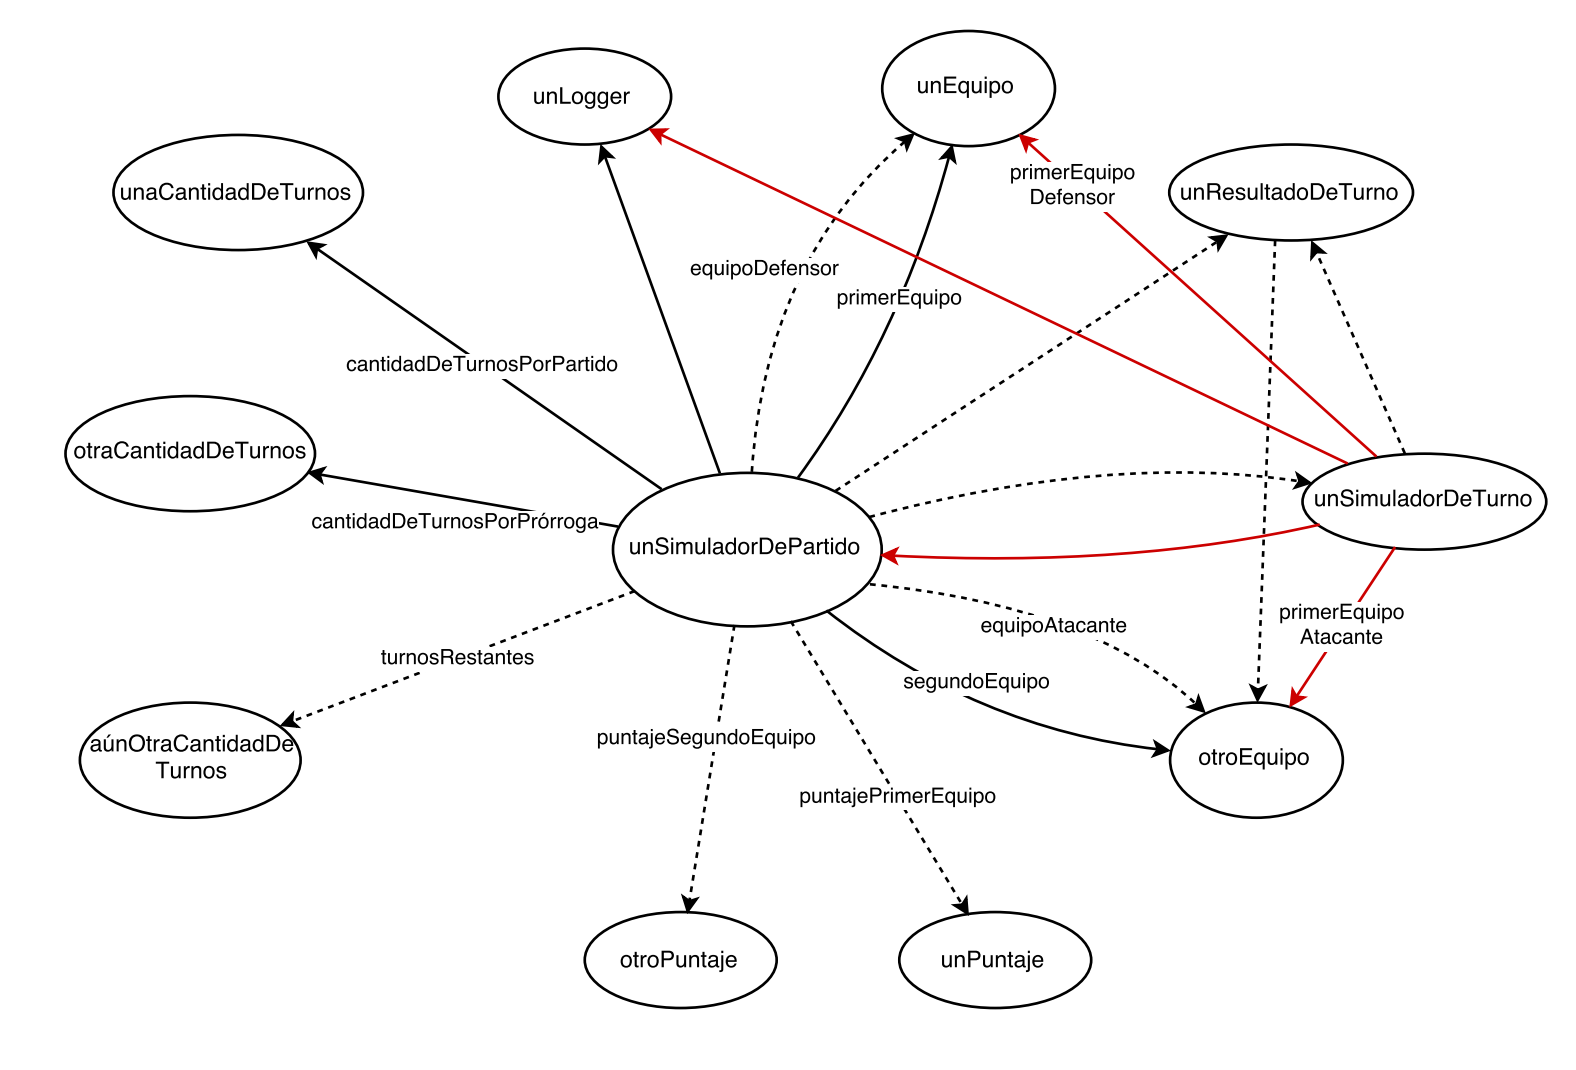
\includegraphics[width=15cm]{diagramas/DO1}
\end{center}

Diagrama de objetos luego de actualizar el simulador de partido.

\begin{center}
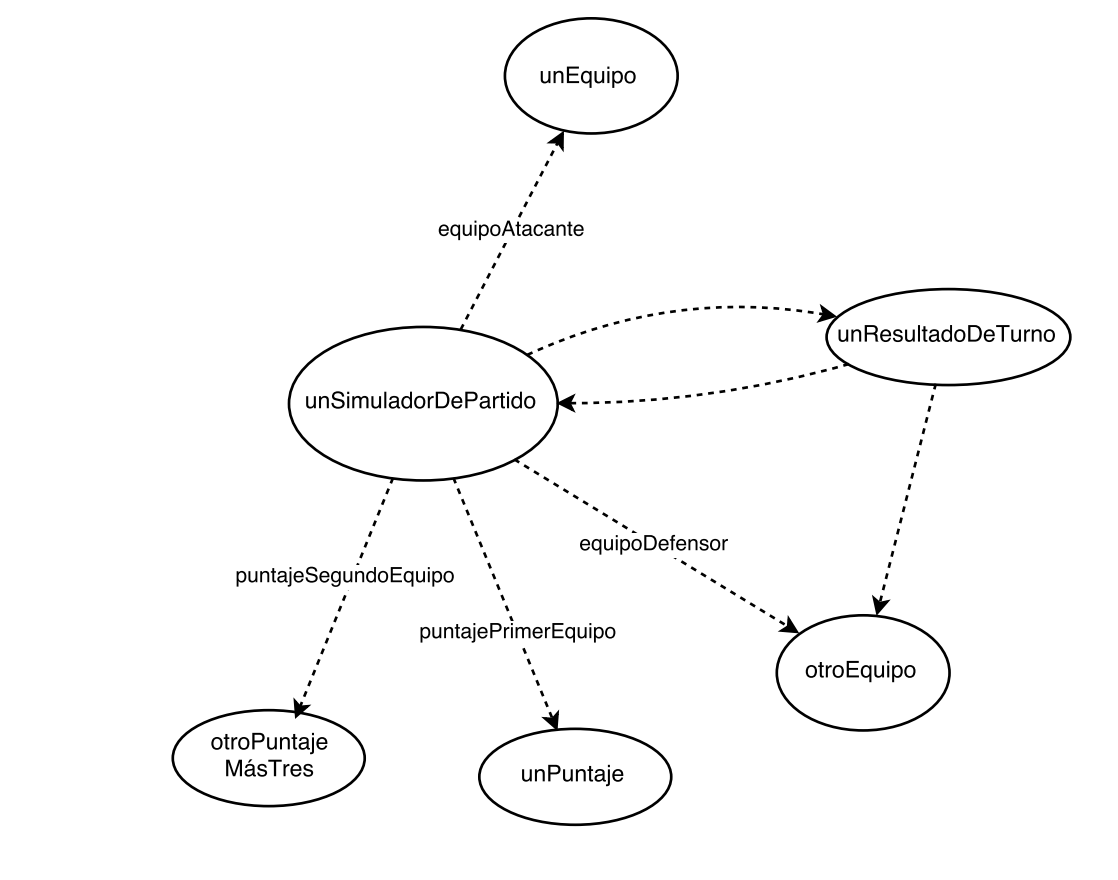
\includegraphics[width=15cm]{diagramas/DO2}
\end{center}

\subsubsection{Simulador de Turno}

Diagrama de objetos de un simulador de turnos, para el caso en que una jugada termina en pase robado, justo antes que el resultado de la jugada actualice el simulador de turno.

\begin{center}
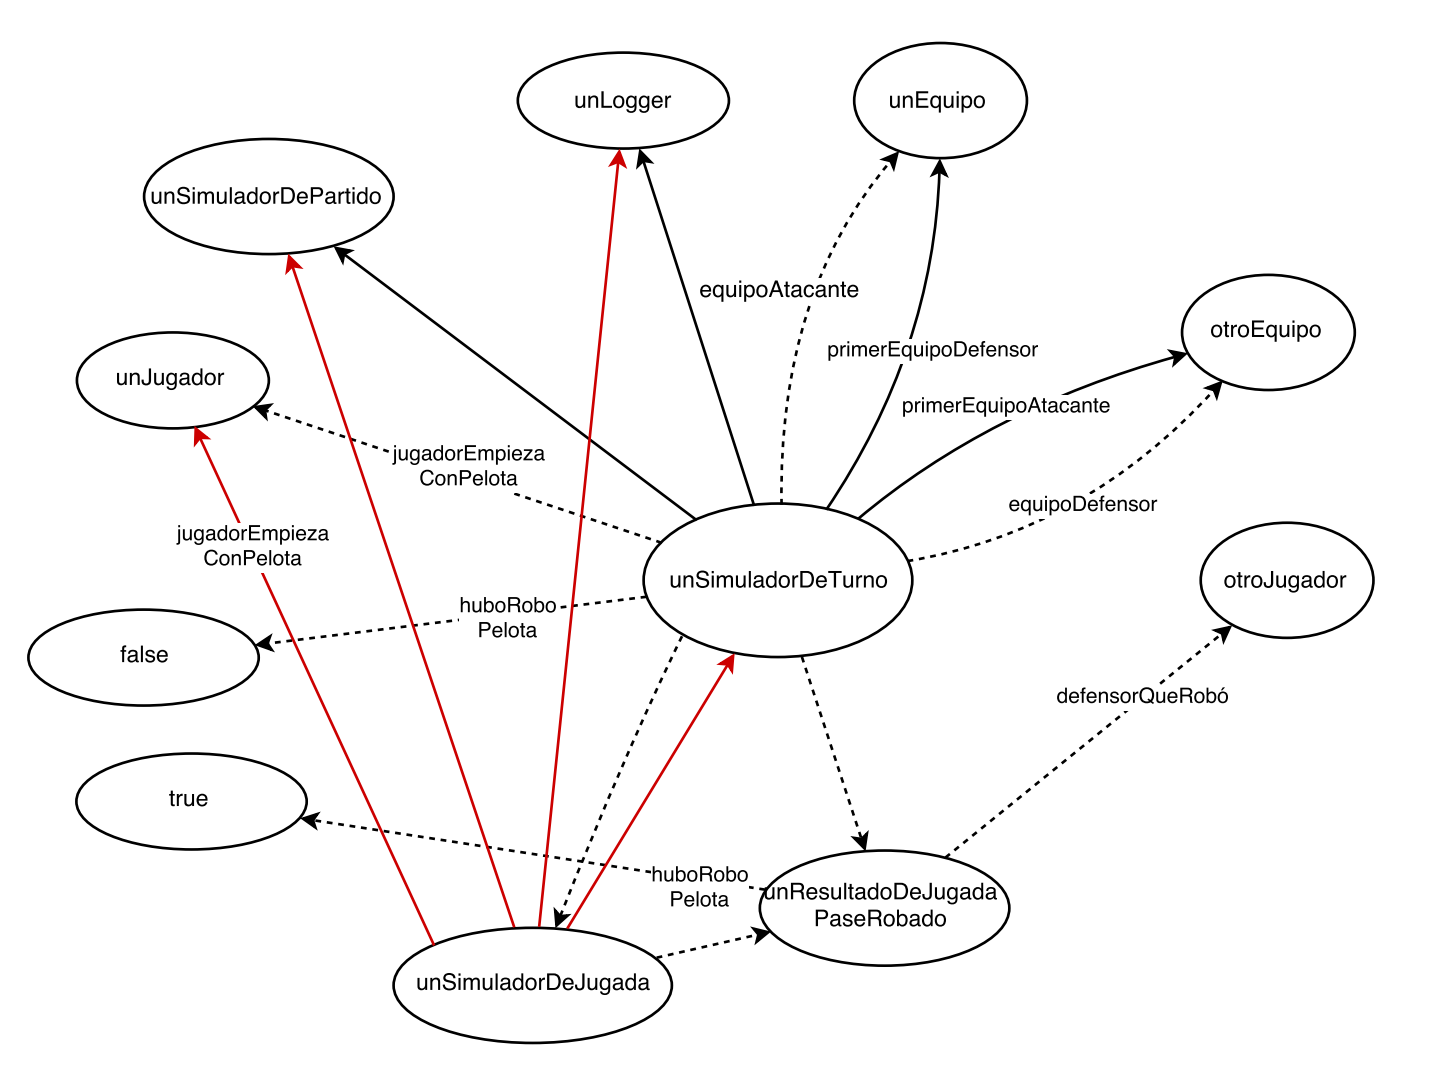
\includegraphics[width=15cm]{diagramas/DO3}
\end{center}

Diagrama de objetos luego de actualizar el turno.

\begin{center}
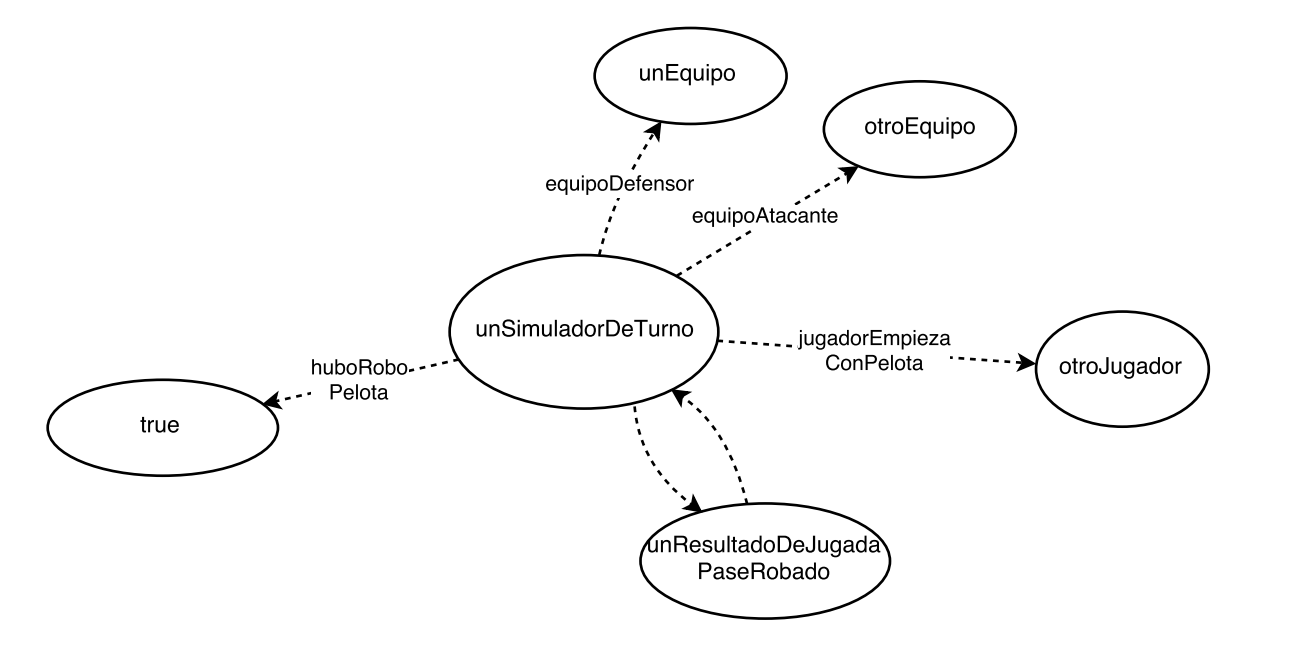
\includegraphics[width=15cm]{diagramas/DO4}
\end{center}

Diagrama de objetos luego de la \'ultima jugada del turno.

\begin{center}
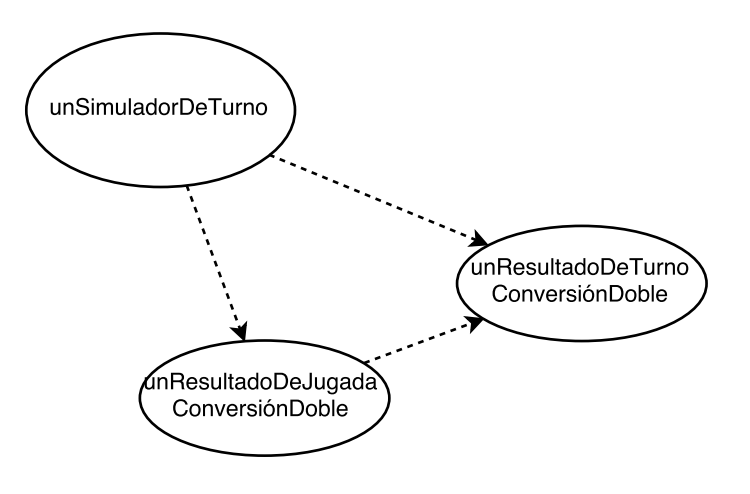
\includegraphics[width=8cm]{diagramas/DO5}
\end{center}

\subsubsection{Simulador de Jugada}

Diagrama de objetos de un simulador de jugada, para el caso en que un momento termina en pase exitoso, justo antes que el resultado del momento
actualice el simulador de jugada.

\begin{center}
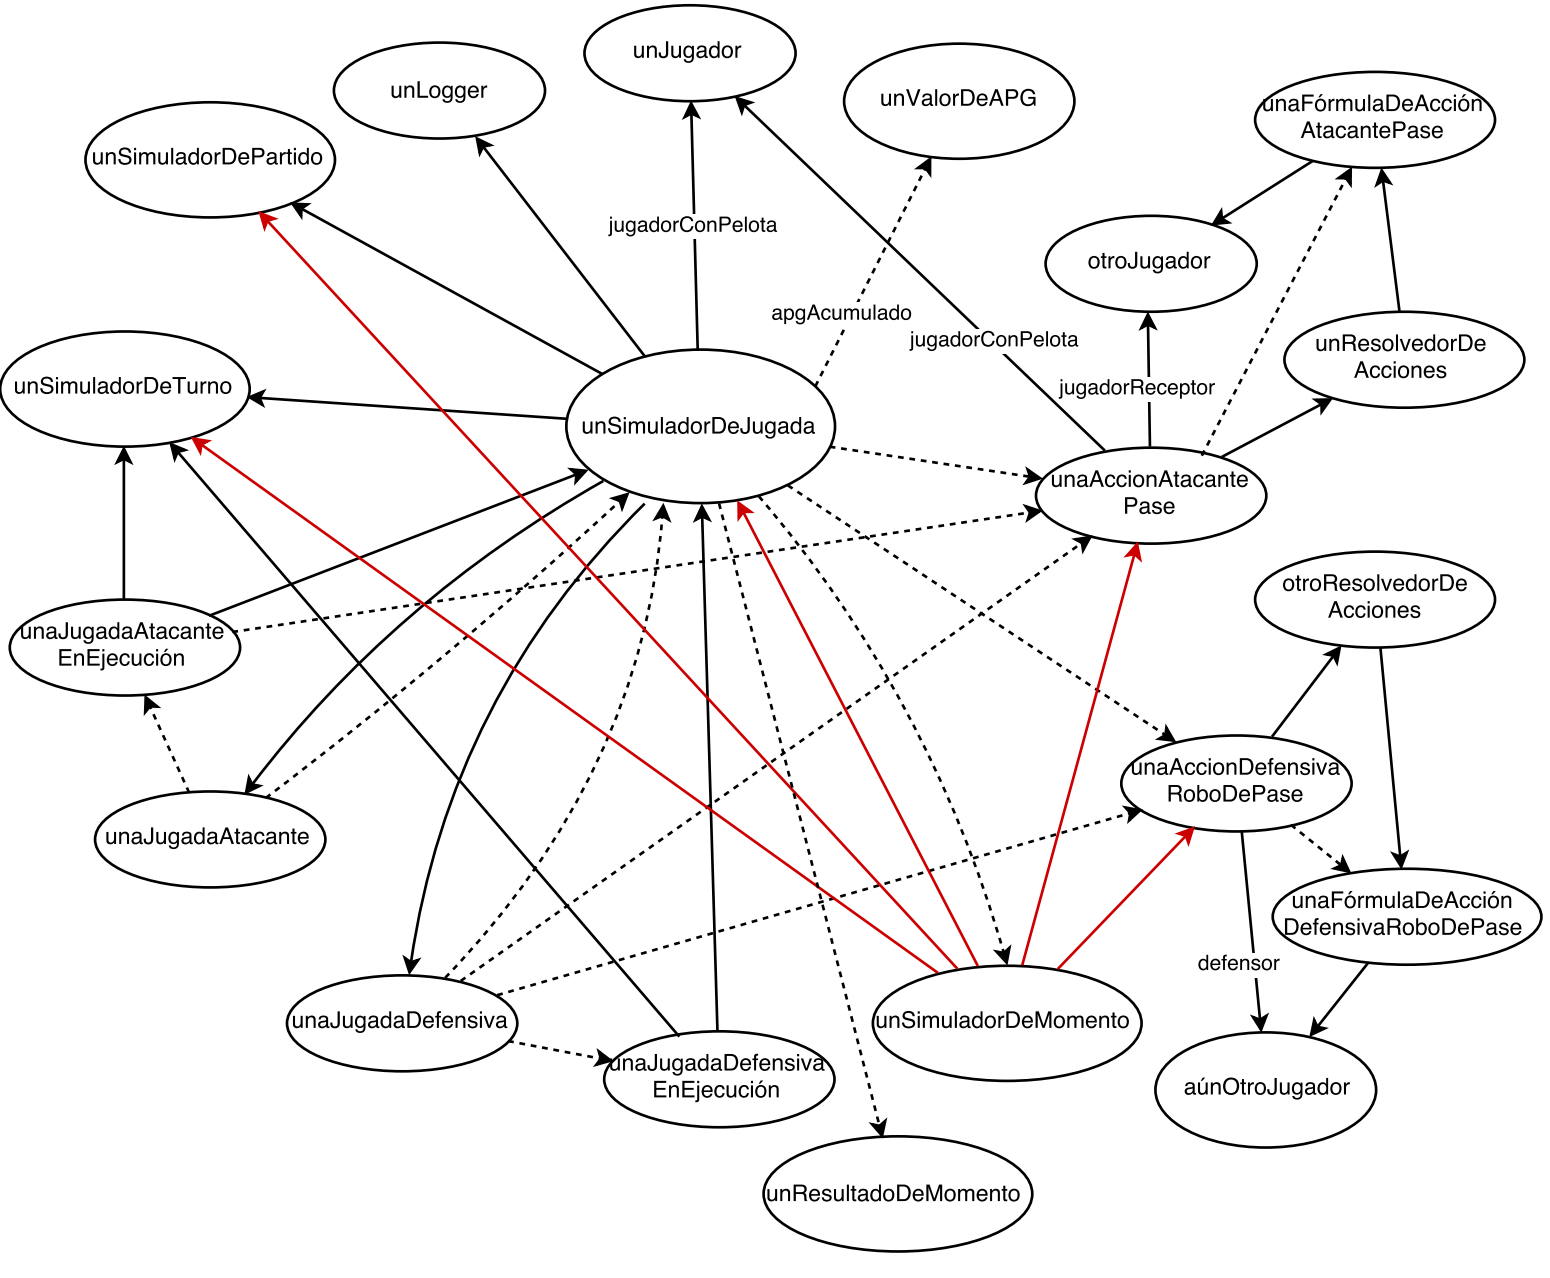
\includegraphics[width=15cm]{diagramas/DO6}
\end{center}

Diagrama de objetos luego de actualizar el simulador de jugada.

\begin{center}
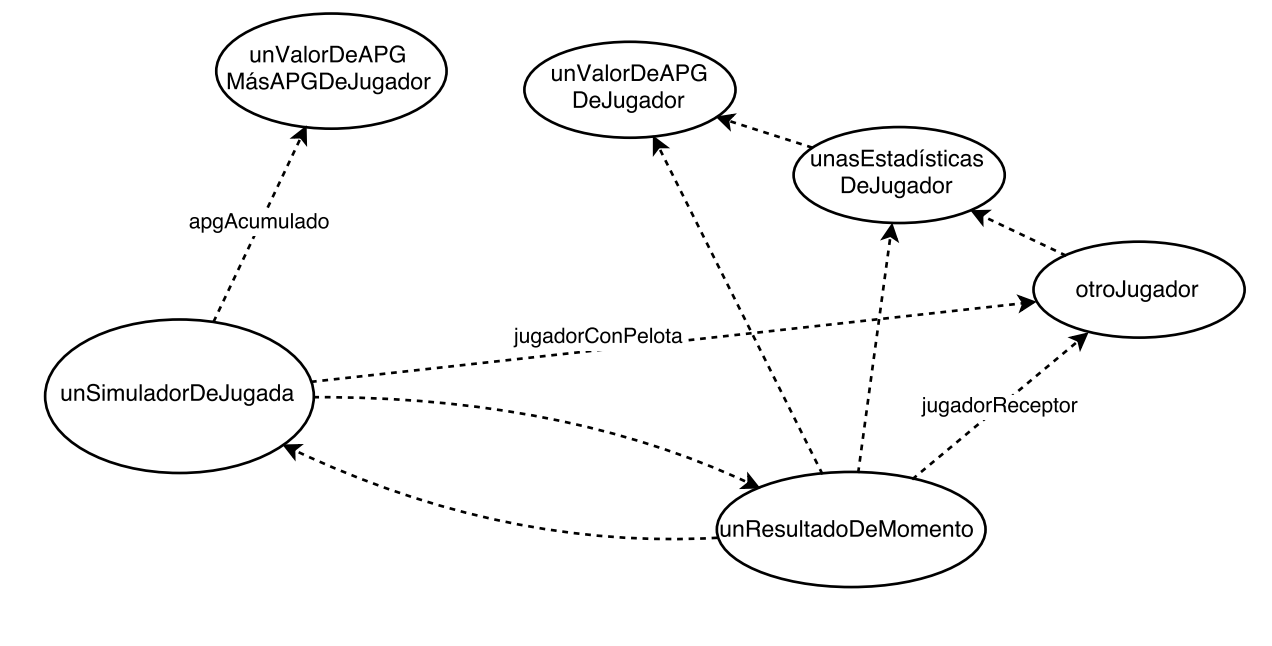
\includegraphics[width=15cm]{diagramas/DO7}
\end{center}

\subsubsection{Simulador de Momento}

Diagrama de objetos de un simulador de momento, para el caso de un pase fallido por robo de pelota.

\begin{center}
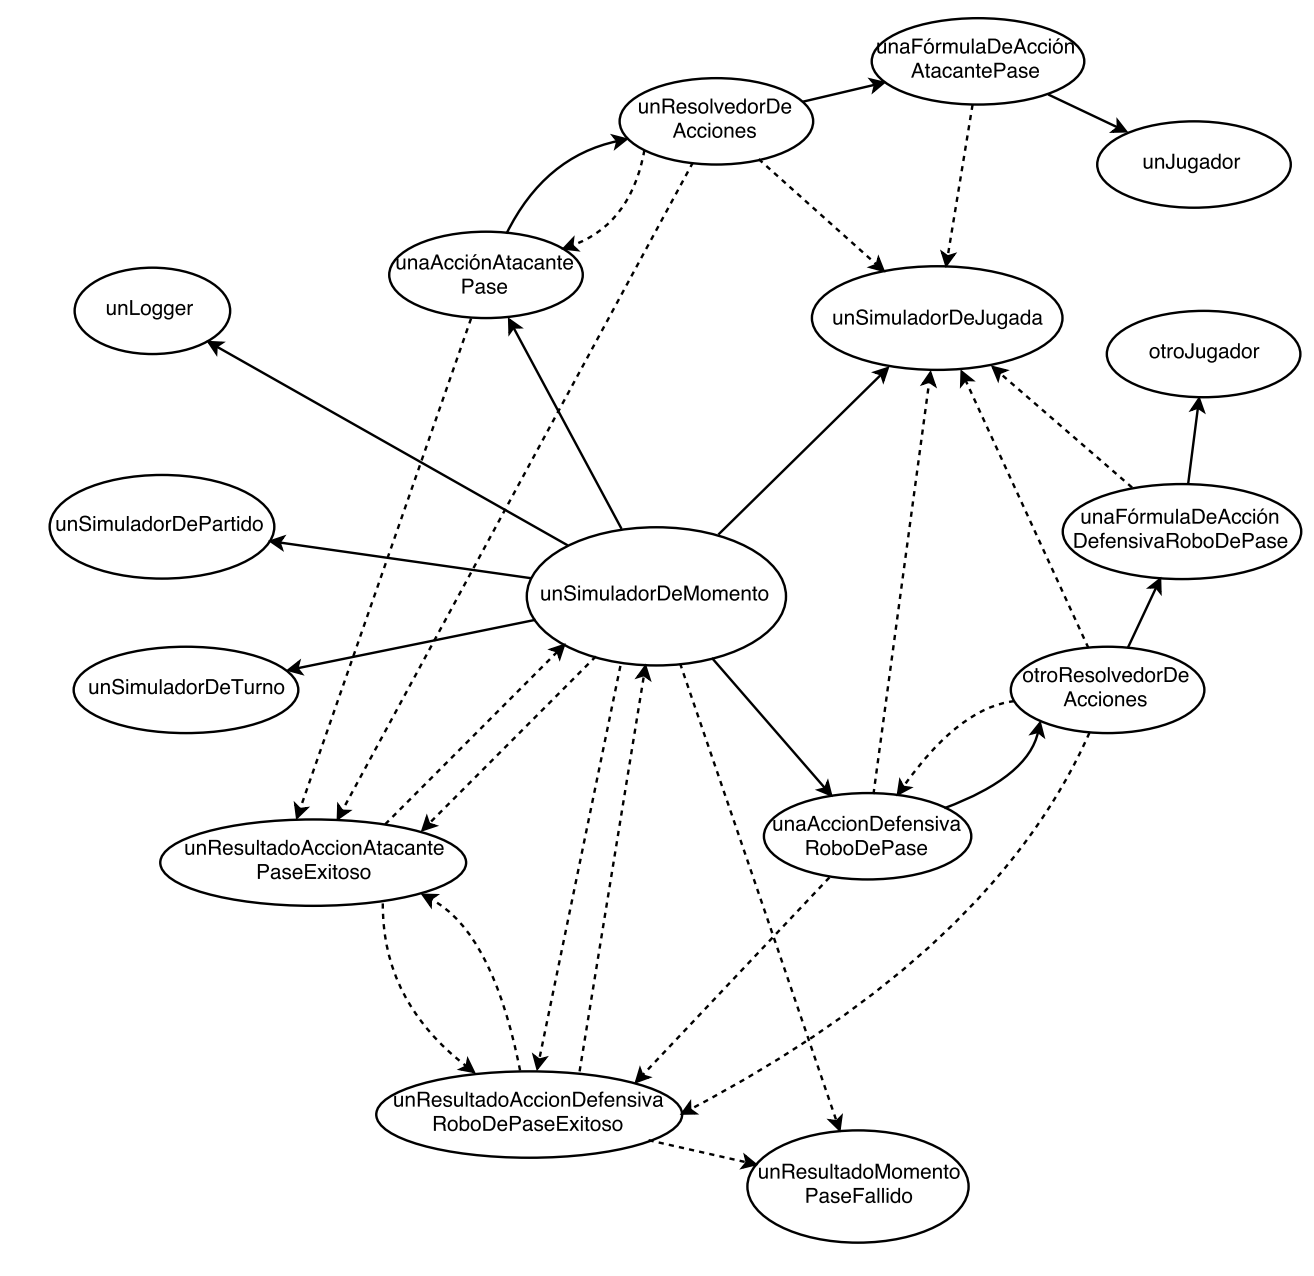
\includegraphics[width=15cm]{diagramas/DO8}
\end{center}

\subsection{Diagrama de secuencia}
% presentación de la razón de ser
Incluimos un diagrama de secuencia que abarca la secuencia de colaboraciones que desencadena el envío
del mensaje jugar (simular, finalmente) a la clase SimuladorMomento con el objetivo de mostrar claramente
la interacción mediante la cual se resuelven las acciones atacantes y defensivas en un Momento particular.

% explicación del diagrama
El diagrama muestra que para simular un MomentoDeJugada se deben obtener el resultado de simular ambas acciones
utilizando las fórmulas de resolución de acciones, ofensiva y defensiva, independientemente. Una vez definido el resultado de
cada una de las acciones mediante un double dispatch se obtiene el resultado del momento. El double dispatch se realiza entre
el resultado de la acción atacante al cual se le envia el mensaje obtenerResultadoMomento recibiendo como colaborador externo
al resultado de la acción defensiva. El resultado de la acción atacante invoca el mensaje correspondiente sobre el resultado de
la acción defensiva en función de su propio tipo. Finalmente, el resultado de acción defensiva devolverá el resultado del momento
en función de su propio tipo, completando el double dispatch.

\begin{center}
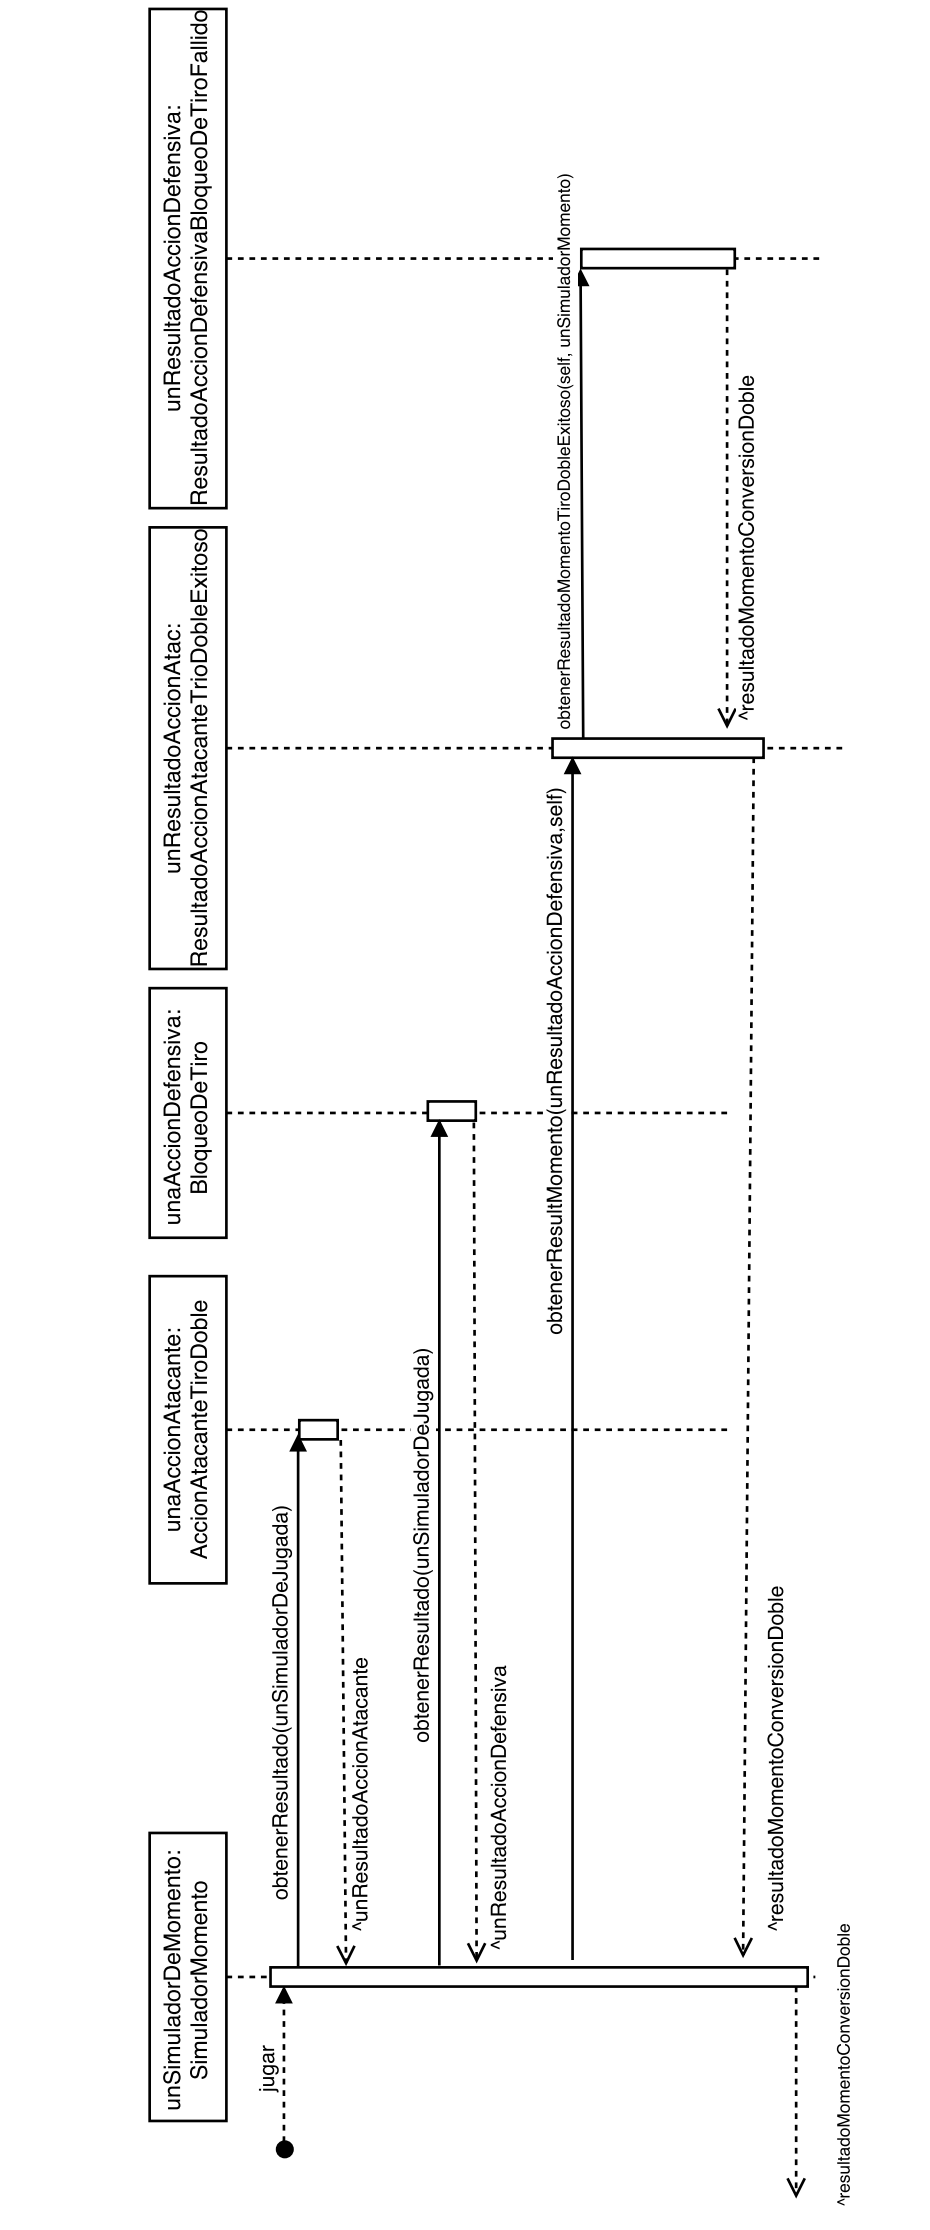
\includegraphics[width=8cm]{diagramas/secuencia}
\end{center}

\newpage

\subsection{Diagramas de clase}

El correspondiente diagrama de clases lo enviamos adjunto con el informe a causa del tamaño del gr\'afico. A continuación, realizamos un par de aclaraciones sobre el g\'afico:

\begin{enumerate}
  \item Agregamos clases en color verde, estas clases son clases replicadas, es decir, clases que duplicamos para hacer mas legible el diagrama.
  \item Los conectores de herencia estan hechos con flechas de tamaño mas grande que las comunes, de esta forma el diagrama es mas legible.
\end{enumerate}


\section{Burndown}

A continuaci\'on mostramos el diagrama Burndown, el cual se utiliza para graficar el trabajo pendiente; en particular, la cantidad de horas pendientes del proyecto a lo largo del tiempo.
En el gr\'afico vemos la recta azul que simboliza un progreso equitativo y cumpliendo las horas propuestas, y en rojo vemos la curva real. Idealmente, la curva que describe la realidad se parecer\'ia lo m\'as posible a la lineal.

Analizando el gr\'afico podemos ver que el proyecto se llev\'o adelante a un ritmo que se aproxima a un ritmo lineal, a excepci\'on de algunos picos donde se demor\'o el desarrollo, pero luego convergió al resultado esperado.

  \begin{center}
	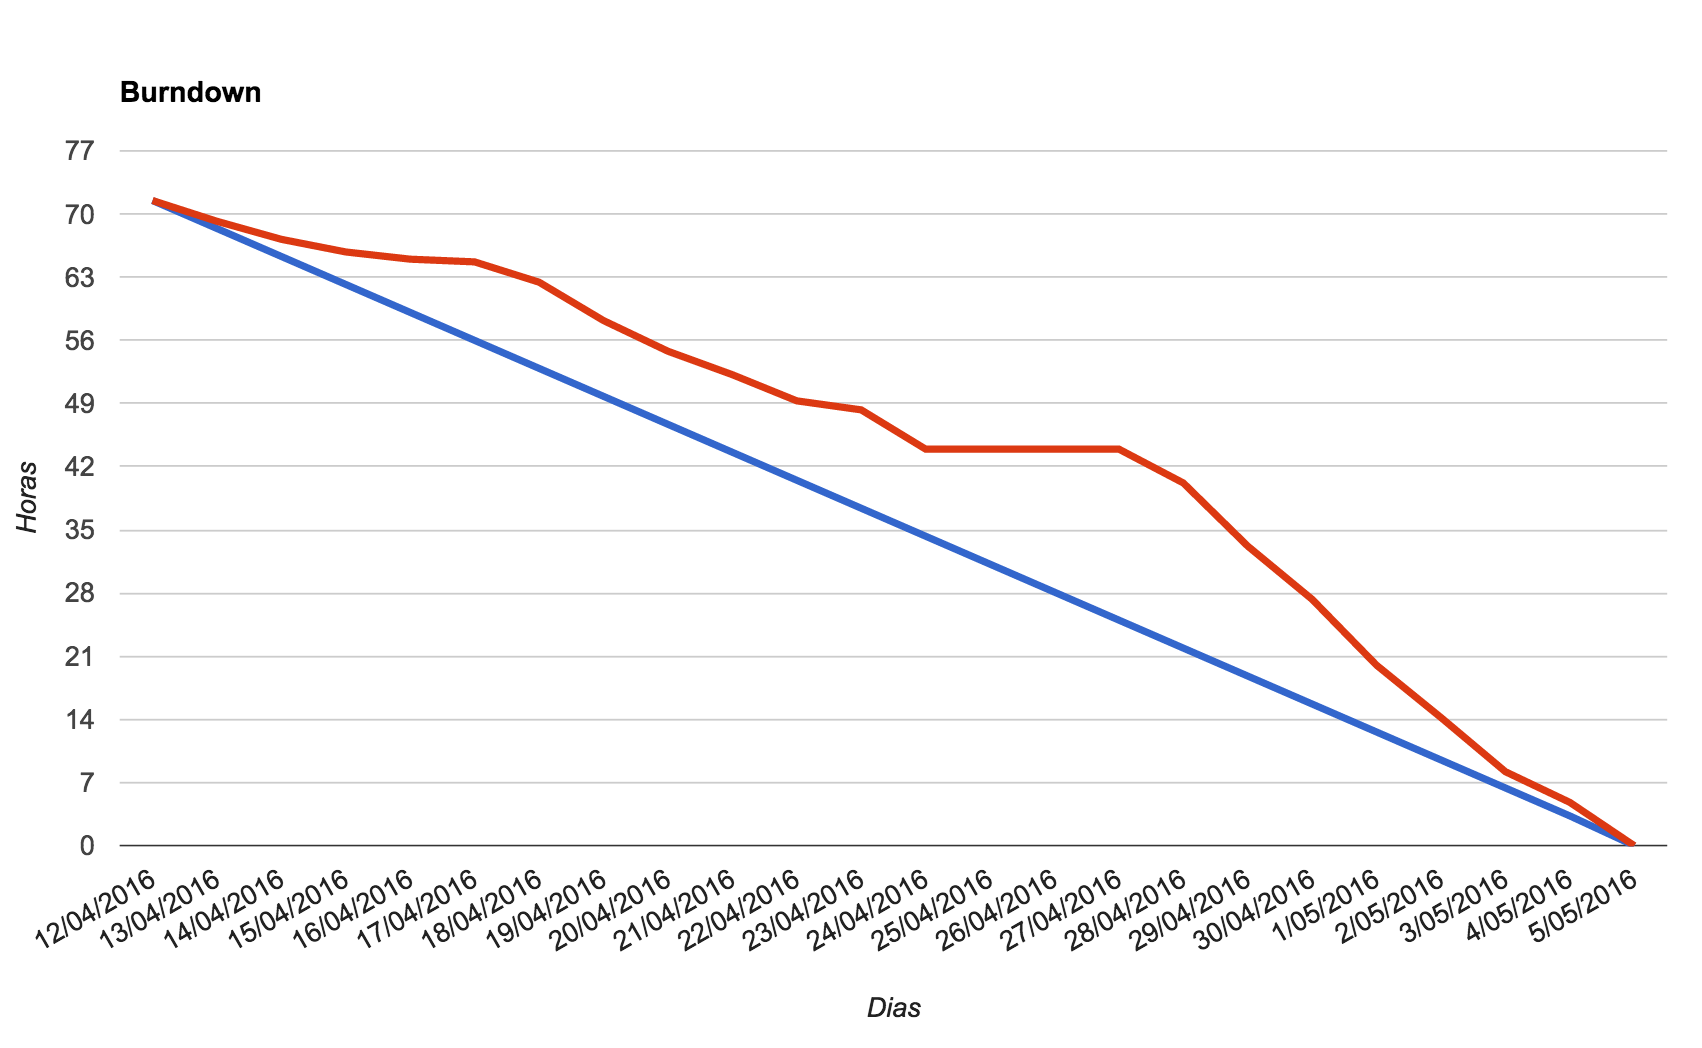
\includegraphics[width=15cm]{diagramas/burn}
  \end{center}
\section{Conclusi'on}

% opinión retrospectiva sobre las herramientas
El desarrollo del sistema nos facilitó la apreciación de la utilidad de varias de las herramientas
que usamos como los gráficos y las heurísticas de diseño. Sin embargo, en varios momentos
el orden en el que realizamos las tareas consideramos que nos perjudicó. Por ejemplo, el
subdividir el trabajo en stories sin haber pensado en el diseño del sistema antes, produjo
una correspondencia pobre entre las stories que habíamos definido y las tareas que finalmente
tuvimos que realizar.

% desafíos
Los gráficos resultaron ser una buena base para discutir las opciones de diseño de forma barata
sin tener que invertir el tiempo que hubiera tomado programar cada una de las alternativas. Sin embargo,
sucedió varias veces que no nos percatábamos de ciertos problemas hasta que no los implementábamos.
Además, uno de los mayores desafíos que encontramos en el TP fue pensar diseños que satisfacieran
todas las heurísticas de diseño que teníamos presentes (alta cohesión, bajo acoplamiento, alta modularidad, etc.).
La mayoría de las veces tuvimos que evaluar las ventajas y desventajas de cada alternativa para finalmente 
decidir la que nos pareciera mejor para la circunstancia particular y los posibles ejes de cambio.

% target process
Finalmente, nos gustaría comentar que la utilización de la herramienta de Scrum Target Process no nos 
pareció que nos ayudara a organizarnos o mejorar. Probablemente esto se deba a que el proyecto fue demasiado
corto para poder utilizar las herramientas de seguimiento de Target Process durante las retrospectivas
y organizarnos mejor.


\end{document}
